% =====================================================================
% AUTO-GENERATED from docs/erw-model.md by docs/build-erw-model.sh.
% Do NOT edit this file directly — your changes will be overwritten on
% the next rebuild. Edit erw-model.md and re-run build-erw-model.sh.
% =====================================================================
% Options for packages loaded elsewhere
\PassOptionsToPackage{unicode}{hyperref}
\PassOptionsToPackage{hyphens}{url}
\PassOptionsToPackage{dvipsnames,svgnames,x11names}{xcolor}
\documentclass[
  11pt,
]{article}
\usepackage{xcolor}
\usepackage[margin=2.3cm]{geometry}
\usepackage{amsmath,amssymb}
\setcounter{secnumdepth}{-\maxdimen} % remove section numbering
\usepackage{iftex}
\ifPDFTeX
  \usepackage[T1]{fontenc}
  \usepackage[utf8]{inputenc}
  \usepackage{textcomp} % provide euro and other symbols
\else % if luatex or xetex
  \usepackage{unicode-math} % this also loads fontspec
  \defaultfontfeatures{Scale=MatchLowercase}
  \defaultfontfeatures[\rmfamily]{Ligatures=TeX,Scale=1}
\fi
\usepackage{lmodern}
\ifPDFTeX\else
  % xetex/luatex font selection
  \setmainfont[]{Helvetica Neue}
  \setmonofont[]{Menlo}
\fi
% Use upquote if available, for straight quotes in verbatim environments
\IfFileExists{upquote.sty}{\usepackage{upquote}}{}
\IfFileExists{microtype.sty}{% use microtype if available
  \usepackage[]{microtype}
  \UseMicrotypeSet[protrusion]{basicmath} % disable protrusion for tt fonts
}{}
\makeatletter
\@ifundefined{KOMAClassName}{% if non-KOMA class
  \IfFileExists{parskip.sty}{%
    \usepackage{parskip}
  }{% else
    \setlength{\parindent}{0pt}
    \setlength{\parskip}{6pt plus 2pt minus 1pt}}
}{% if KOMA class
  \KOMAoptions{parskip=half}}
\makeatother
\usepackage{color}
\usepackage{fancyvrb}
\newcommand{\VerbBar}{|}
\newcommand{\VERB}{\Verb[commandchars=\\\{\}]}
\DefineVerbatimEnvironment{Highlighting}{Verbatim}{commandchars=\\\{\}}
% Add ',fontsize=\small' for more characters per line
\newenvironment{Shaded}{}{}
\newcommand{\AlertTok}[1]{\textcolor[rgb]{1.00,0.00,0.00}{\textbf{#1}}}
\newcommand{\AnnotationTok}[1]{\textcolor[rgb]{0.38,0.63,0.69}{\textbf{\textit{#1}}}}
\newcommand{\AttributeTok}[1]{\textcolor[rgb]{0.49,0.56,0.16}{#1}}
\newcommand{\BaseNTok}[1]{\textcolor[rgb]{0.25,0.63,0.44}{#1}}
\newcommand{\BuiltInTok}[1]{\textcolor[rgb]{0.00,0.50,0.00}{#1}}
\newcommand{\CharTok}[1]{\textcolor[rgb]{0.25,0.44,0.63}{#1}}
\newcommand{\CommentTok}[1]{\textcolor[rgb]{0.38,0.63,0.69}{\textit{#1}}}
\newcommand{\CommentVarTok}[1]{\textcolor[rgb]{0.38,0.63,0.69}{\textbf{\textit{#1}}}}
\newcommand{\ConstantTok}[1]{\textcolor[rgb]{0.53,0.00,0.00}{#1}}
\newcommand{\ControlFlowTok}[1]{\textcolor[rgb]{0.00,0.44,0.13}{\textbf{#1}}}
\newcommand{\DataTypeTok}[1]{\textcolor[rgb]{0.56,0.13,0.00}{#1}}
\newcommand{\DecValTok}[1]{\textcolor[rgb]{0.25,0.63,0.44}{#1}}
\newcommand{\DocumentationTok}[1]{\textcolor[rgb]{0.73,0.13,0.13}{\textit{#1}}}
\newcommand{\ErrorTok}[1]{\textcolor[rgb]{1.00,0.00,0.00}{\textbf{#1}}}
\newcommand{\ExtensionTok}[1]{#1}
\newcommand{\FloatTok}[1]{\textcolor[rgb]{0.25,0.63,0.44}{#1}}
\newcommand{\FunctionTok}[1]{\textcolor[rgb]{0.02,0.16,0.49}{#1}}
\newcommand{\ImportTok}[1]{\textcolor[rgb]{0.00,0.50,0.00}{\textbf{#1}}}
\newcommand{\InformationTok}[1]{\textcolor[rgb]{0.38,0.63,0.69}{\textbf{\textit{#1}}}}
\newcommand{\KeywordTok}[1]{\textcolor[rgb]{0.00,0.44,0.13}{\textbf{#1}}}
\newcommand{\NormalTok}[1]{#1}
\newcommand{\OperatorTok}[1]{\textcolor[rgb]{0.40,0.40,0.40}{#1}}
\newcommand{\OtherTok}[1]{\textcolor[rgb]{0.00,0.44,0.13}{#1}}
\newcommand{\PreprocessorTok}[1]{\textcolor[rgb]{0.74,0.48,0.00}{#1}}
\newcommand{\RegionMarkerTok}[1]{#1}
\newcommand{\SpecialCharTok}[1]{\textcolor[rgb]{0.25,0.44,0.63}{#1}}
\newcommand{\SpecialStringTok}[1]{\textcolor[rgb]{0.73,0.40,0.53}{#1}}
\newcommand{\StringTok}[1]{\textcolor[rgb]{0.25,0.44,0.63}{#1}}
\newcommand{\VariableTok}[1]{\textcolor[rgb]{0.10,0.09,0.49}{#1}}
\newcommand{\VerbatimStringTok}[1]{\textcolor[rgb]{0.25,0.44,0.63}{#1}}
\newcommand{\WarningTok}[1]{\textcolor[rgb]{0.38,0.63,0.69}{\textbf{\textit{#1}}}}
\usepackage{longtable,booktabs,array}
\newcounter{none} % for unnumbered tables
\usepackage{calc} % for calculating minipage widths
% Correct order of tables after \paragraph or \subparagraph
\usepackage{etoolbox}
\makeatletter
\patchcmd\longtable{\par}{\if@noskipsec\mbox{}\fi\par}{}{}
\makeatother
% Allow footnotes in longtable head/foot
\IfFileExists{footnotehyper.sty}{\usepackage{footnotehyper}}{\usepackage{footnote}}
\makesavenoteenv{longtable}
\usepackage{graphicx}
\makeatletter
\newsavebox\pandoc@box
\newcommand*\pandocbounded[1]{% scales image to fit in text height/width
  \sbox\pandoc@box{#1}%
  \Gscale@div\@tempa{\textheight}{\dimexpr\ht\pandoc@box+\dp\pandoc@box\relax}%
  \Gscale@div\@tempb{\linewidth}{\wd\pandoc@box}%
  \ifdim\@tempb\p@<\@tempa\p@\let\@tempa\@tempb\fi% select the smaller of both
  \ifdim\@tempa\p@<\p@\scalebox{\@tempa}{\usebox\pandoc@box}%
  \else\usebox{\pandoc@box}%
  \fi%
}
% Set default figure placement to htbp
\def\fps@figure{htbp}
\makeatother
\setlength{\emergencystretch}{3em} % prevent overfull lines
\providecommand{\tightlist}{%
  \setlength{\itemsep}{0pt}\setlength{\parskip}{0pt}}
% Header includes for docs/erw-model.tex (injected by build-erw-model.sh).
% Tighten longtable layout so wide tables with monospace cells fit on A4.
\usepackage{etoolbox}
\setlength{\tabcolsep}{4pt}
\renewcommand{\arraystretch}{1.05}
% Allow line breaks inside long \texttt{} strings (filenames, paths)
\usepackage{seqsplit}
% Inside longtable cells: shrink font and let \texttt{} break anywhere so long
% filenames (e.g. cdr_{climate_factor,pedogenic_fraction,per_t_basalt}.tif)
% wrap inside narrow columns instead of overflowing the page. seqsplit only
% inserts breakpoints — no visual effect unless a break is actually needed.
\protected\def\erwBreakableTexttInTables{%
  \let\origtexttt\texttt
  \def\texttt##1{\origtexttt{\seqsplit{##1}}}%
}
\AtBeginEnvironment{longtable}{\footnotesize\erwBreakableTexttInTables}
% Give the paragraph builder room to stretch before resorting to overfull lines.
\setlength{\emergencystretch}{3em}
\usepackage{bookmark}
\IfFileExists{xurl.sty}{\usepackage{xurl}}{} % add URL line breaks if available
\urlstyle{same}
\hypersetup{
  colorlinks=true,
  linkcolor={NavyBlue},
  filecolor={Maroon},
  citecolor={Blue},
  urlcolor={NavyBlue},
  pdfcreator={LaTeX via pandoc}}

\title{Ex-Ante ERW Model --- Living Documentation}
\usepackage{etoolbox}
\makeatletter
\providecommand{\subtitle}[1]{% add subtitle to \maketitle
  \apptocmd{\@title}{\par {\large #1 \par}}{}{}
}
\makeatother
\subtitle{Geospatial profitability model for Enhanced Rock Weathering with basalt in Sub-Saharan Africa}
\author{}
\date{2026-05-26}

\begin{document}
\maketitle

{
\hypersetup{linkcolor=NavyBlue}
\setcounter{tocdepth}{3}
\tableofcontents
}
\section{Ex-Ante ERW Model --- Living
Documentation}\label{ex-ante-erw-model-living-documentation}

\textbf{Geospatial profitability model for Enhanced Rock Weathering with
basalt in Sub-Saharan Africa.} This document is the single source of
truth for the \emph{current} state of the model. Update it whenever
anything material changes --- the \textbf{Status at a glance} section,
the \textbf{Changelog}, the affected block under §6, and the affected
output under §7.

Companion documents that this file points to (do not duplicate):

{\def\LTcaptype{none} % do not increment counter
\begin{longtable}[]{@{}
  >{\raggedright\arraybackslash}p{(\linewidth - 2\tabcolsep) * \real{0.5000}}
  >{\raggedright\arraybackslash}p{(\linewidth - 2\tabcolsep) * \real{0.5000}}@{}}
\toprule\noalign{}
\begin{minipage}[b]{\linewidth}\raggedright
File
\end{minipage} & \begin{minipage}[b]{\linewidth}\raggedright
Purpose
\end{minipage} \\
\midrule\noalign{}
\endhead
\bottomrule\noalign{}
\endlastfoot
\texttt{docs/erw-review.md} & Evidence review (literature on ERW
chemistry, feedstocks, trials, agronomy, risks). \\
\texttt{docs/erw-parameters.md} & Catalogue of every constant and
assumption with citations and units. \\
\texttt{docs/erw-README.md} & Runbook: file inventory, run order, output
schema, known portability issues. \\
\texttt{docs/erw-conceptual-framework.\{svg,pdf,tex\}} & Scientific
framework figure --- three streams converging on the gross-margin
equation. \\
\texttt{docs/erw-pipeline-flow.\{svg,pdf,tex\}} & Pipeline architecture
figure --- how the code implements the framework. \\
\texttt{docs/maps/*.png} & Rendered indicator and outcome maps (12
currently). \\
\texttt{flows.html} & Browser-rendered view of this whole thing. \\
\end{longtable}
}

\begin{center}\rule{0.5\linewidth}{0.5pt}\end{center}

\subsection{0. Status at a glance}\label{status-at-a-glance}

\textbf{Last updated:} 2026-05-26 \textbf{Geographic scope:} Sub-Saharan
Africa, 47 countries, GADM v4 boundaries \textbf{Working grid:}
SoilGrids-Africa 30 arc-sec aggregated 10× → \textasciitilde0.083° (≈9
km) --- 746 × 828 cells \textbf{Currency:} USD; \textbf{CO₂ in tonnes;
year-1 / NPV @ 10\% / equilibrium regimes} \textbf{Defaults (refreshed
2026-05-26):} grain size \textbf{50 µm}, MRV \textbf{\$20 / tCO₂},
year-1 agronomic return \textbf{summed over 5-yr basalt residency},
pedogenic deduction via \textbf{CGIAR-CSI Global Aridity Index}, EcoCrop
max-pH cliff \textbf{per-crop optima (5.5--8.0)}.

\subsubsection{Pipeline-block status}\label{pipeline-block-status}

{\def\LTcaptype{none} % do not increment counter
\begin{longtable}[]{@{}
  >{\raggedright\arraybackslash}p{(\linewidth - 6\tabcolsep) * \real{0.2500}}
  >{\raggedright\arraybackslash}p{(\linewidth - 6\tabcolsep) * \real{0.2500}}
  >{\raggedright\arraybackslash}p{(\linewidth - 6\tabcolsep) * \real{0.2500}}
  >{\raggedright\arraybackslash}p{(\linewidth - 6\tabcolsep) * \real{0.2500}}@{}}
\toprule\noalign{}
\begin{minipage}[b]{\linewidth}\raggedright
Block
\end{minipage} & \begin{minipage}[b]{\linewidth}\raggedright
Stage(s)
\end{minipage} & \begin{minipage}[b]{\linewidth}\raggedright
Status
\end{minipage} & \begin{minipage}[b]{\linewidth}\raggedright
Notes
\end{minipage} \\
\midrule\noalign{}
\endhead
\bottomrule\noalign{}
\endlastfoot
B1. Working grid & \texttt{erw-1}, \texttt{erw-2} & \textbf{REAL} &
SoilGrids properties + SPAM v2 (23 crops) co-registered on the 10×
grid \\
B2. Basalt rate & \texttt{erw-3} & \textbf{REAL} & LiTAS / Kamprath /
Cochrane / maintenance + uniform 10/20/50 t·ha⁻¹ \\
B3. CDR surface & \texttt{erw-9} & \textbf{REAL} (refreshed 2026-05-26)
& Climate × pH × pedogenic-C deduction; now consumes CGIAR-CSI AI when
present (else MAP fallback); 50 µm grain default; mean cumulative CDR
under LiTAS-targeted 3.5 t CO₂/ha. \\
B4. Logistics & \texttt{erw-basalt-access} & \textbf{REAL} (since
2026-05-15) & Friction surface fetched, mask expanded to vb+pb,
end-to-end delivered price computed \\
B5. Energy & \texttt{erw-energy-country} & \textbf{REAL} & Country
tariff + grid CI rasters \\
B6. Crop response --- EcoCrop & \texttt{erw-4}, \texttt{erw-5} &
\textbf{REAL} (refreshed 2026-05-26) & Per-crop max\_ph cliffs (5.5 tea
→ 8.0 chickpea, was flat 5.5); all 23 crops × 2 responses \\
B6. Crop response --- Bayesian & \texttt{erw-yield-fit},
\texttt{erw-yield-predict} & \textbf{NOT RUN} & Trial-anchored brms
model not fit; erw-7 falls back to EcoCrop \\
B7. Profitability & \texttt{erw-7} & \textbf{REAL} (refreshed
2026-05-26) & 276 gross-margin rasters; year-1 regime now sums agronomic
return over 5-yr horizon; MRV \$30 → \$20 \\
B8. Supply ranking & \texttt{erw-supply} & \textbf{REAL} (refreshed
2026-05-26) & Three supply curves + nine deployment masks; year-1 peak
GM \$19.6B @ 250 Mt/yr; NPV peak \$5.0B @ 100 Mt/yr \\
B9. Sensitivity & \texttt{erw-8} & \textbf{READY} & Variable-name bug
patched 2026-05-19; not yet re-run at the new defaults; default-scope
sweep is ≈6--8 h wall time \\
\end{longtable}
}

\subsubsection{Headline numbers (current
run)}\label{headline-numbers-current-run}

{\def\LTcaptype{none} % do not increment counter
\begin{longtable}[]{@{}
  >{\raggedright\arraybackslash}p{(\linewidth - 4\tabcolsep) * \real{0.3333}}
  >{\raggedright\arraybackslash}p{(\linewidth - 4\tabcolsep) * \real{0.3333}}
  >{\raggedright\arraybackslash}p{(\linewidth - 4\tabcolsep) * \real{0.3333}}@{}}
\toprule\noalign{}
\begin{minipage}[b]{\linewidth}\raggedright
Metric
\end{minipage} & \begin{minipage}[b]{\linewidth}\raggedright
Value
\end{minipage} & \begin{minipage}[b]{\linewidth}\raggedright
Source raster / table
\end{minipage} \\
\midrule\noalign{}
\endhead
\bottomrule\noalign{}
\endlastfoot
Mafic source pixels (vb+pb in SSA) & \textbf{1,399,005} (1.9 \% of SSA
cropland-context cells) & \texttt{basalt\_source\_mask.tif} \\
Mean delivered basalt price & \textbf{\$40.8 / t} (range \$10 -- \$50,
cap binds for \textasciitilde half of pixels) &
\texttt{basalt\_delivered\_price\_usd\_t.tif} \\
Mean travel time to source & \textbf{815 min} (capped at 1000 min ≈ 1000
km @ 60 km/h) & \texttt{basalt\_traveltime\_min.tif} \\
Delivered basalt incl.~grinding + spreading &
\textbf{\textasciitilde\$53 / t mean} (slightly higher than 100 µm due
to grinding cost +\$1/t) & \texttt{erw-7} setup print \\
Per-tonne CDR at reference climate & \textbf{88 kg CO₂ / t basalt} (was
62 at 100 µm) & \texttt{basalt\_feedstock\_chemistry.csv} \\
Mean cumulative CDR (LiTAS-targeted, TAS=0) & \textbf{3.52 t CO₂ / ha}
(was 2.02 t/ha; +74 \%) & \texttt{cdr\_yield\_merlos.tif} \\
Best pixel-mean profitability cell & \textbf{POTA equilibrium targeted
+\$1,984 / ha}; POTA year-1 \$10,560 / ha &
\texttt{economics\_erw/targeted/POTA\_*.tif} \\
Crops with positive pixel-mean GM, targeted & \textbf{Year-1 12/23; NPV
8/23; Equilibrium 19/23} & per-crop summary \\
Break-even supply cap (year-1) & \textbf{≈250 Mt basalt / yr} (marginal
pixel +\$21 / t) & \texttt{supply\_curve\_year1.csv} \\
Break-even supply cap (NPV) & \textbf{≈100 Mt basalt / yr} (marginal
pixel +\$16 / t) & \texttt{supply\_curve\_npv.csv} \\
Break-even supply cap (equilibrium) & \textbf{between 50 and 100 Mt /
yr} (slips +\$20 / t → −\$14 / t) &
\texttt{supply\_curve\_equilibrium.csv} \\
Peak total gross margin (year-1) & \textbf{\$19.6 B at 250 Mt/yr cap}
with 61.0 Mt CDR/yr & \texttt{supply\_curve\_year1.csv} \\
Peak total gross margin (NPV) & \textbf{\$5.0 B at 100 Mt/yr cap} with
27.2 Mt CDR/yr & \texttt{supply\_curve\_npv.csv} \\
Unconstrained SSA capacity (targeted) & \textbf{443 Mt basalt/yr}
(year-1, NPV) / \textbf{145 Mt/yr} (equilibrium maintenance) &
\texttt{supply\_curve\_*.csv} (row \texttt{Inf}) \\
\end{longtable}
}

\subsubsection{Supply curves at a glance --- marginal \$/t basalt vs
annual cap (refreshed
2026-05-26)}\label{supply-curves-at-a-glance-marginal-t-basalt-vs-annual-cap-refreshed-2026-05-26}

{\def\LTcaptype{none} % do not increment counter
\begin{longtable}[]{@{}
  >{\raggedright\arraybackslash}p{(\linewidth - 20\tabcolsep) * \real{0.0909}}
  >{\raggedright\arraybackslash}p{(\linewidth - 20\tabcolsep) * \real{0.0909}}
  >{\raggedright\arraybackslash}p{(\linewidth - 20\tabcolsep) * \real{0.0909}}
  >{\raggedright\arraybackslash}p{(\linewidth - 20\tabcolsep) * \real{0.0909}}
  >{\raggedright\arraybackslash}p{(\linewidth - 20\tabcolsep) * \real{0.0909}}
  >{\raggedright\arraybackslash}p{(\linewidth - 20\tabcolsep) * \real{0.0909}}
  >{\raggedright\arraybackslash}p{(\linewidth - 20\tabcolsep) * \real{0.0909}}
  >{\raggedright\arraybackslash}p{(\linewidth - 20\tabcolsep) * \real{0.0909}}
  >{\raggedright\arraybackslash}p{(\linewidth - 20\tabcolsep) * \real{0.0909}}
  >{\raggedright\arraybackslash}p{(\linewidth - 20\tabcolsep) * \real{0.0909}}
  >{\raggedright\arraybackslash}p{(\linewidth - 20\tabcolsep) * \real{0.0909}}@{}}
\toprule\noalign{}
\begin{minipage}[b]{\linewidth}\raggedright
Regime
\end{minipage} & \begin{minipage}[b]{\linewidth}\raggedright
1 Mt
\end{minipage} & \begin{minipage}[b]{\linewidth}\raggedright
5 Mt
\end{minipage} & \begin{minipage}[b]{\linewidth}\raggedright
10 Mt
\end{minipage} & \begin{minipage}[b]{\linewidth}\raggedright
25 Mt
\end{minipage} & \begin{minipage}[b]{\linewidth}\raggedright
50 Mt
\end{minipage} & \begin{minipage}[b]{\linewidth}\raggedright
\textbf{100 Mt}
\end{minipage} & \begin{minipage}[b]{\linewidth}\raggedright
\textbf{250 Mt}
\end{minipage} & \begin{minipage}[b]{\linewidth}\raggedright
500 Mt
\end{minipage} & \begin{minipage}[b]{\linewidth}\raggedright
Peak total GM (M\$)
\end{minipage} & \begin{minipage}[b]{\linewidth}\raggedright
Peak CDR (Mt)
\end{minipage} \\
\midrule\noalign{}
\endhead
\bottomrule\noalign{}
\endlastfoot
year-1 & +292 & +215 & +186 & +145 & +117 & \textbf{+79} & \textbf{+21}
& −60 & \textbf{19,648 (@250 Mt)} & 61.0 \\
NPV @ 10 \% & +117 & +103 & +86 & +68 & +46 & \textbf{+16} & −16 & −61 &
\textbf{5,018 (@100 Mt)} & 27.2 \\
equilibrium & +197 & +124 & +91 & +45 & +20 & \textbf{−14} & −60 & −60 &
\textbf{3,145 (@100 Mt)} & 24.3 \\
\end{longtable}
}

Values are the marginal pixel's GM per tonne basalt at each supply cap;
bold columns flag the most profitable supply level for each regime. The
year-1 regime now peaks at the 250 Mt/yr cap (\textasciitilde5× the old
peak of \$2 B) thanks to the horizon-summed agronomic return.
Equilibrium saturates at 145 Mt/yr (the targeted-deployable-cropland
ceiling at maintenance rate).

\begin{center}\rule{0.5\linewidth}{0.5pt}\end{center}

\subsection{1. Changelog}\label{changelog}

Reverse chronological. One bullet per material change. Reference the
block(s) affected so it is obvious which section under §6 also moved.

\subsubsection{2026-05-26 --- Round-1 conservatism review; five defaults
re-anchored; B3 / B6 / B7 / B8
re-run}\label{round-1-conservatism-review-five-defaults-re-anchored-b3-b6-b7-b8-re-run}

Outcome of a structural review of the model's conservatism (see also the
``Why we were under-estimating profit'' review below in §8). Five fixes
landed, all backed by the parameter audit and the cited literature:

\begin{itemize}
\tightlist
\item
  \textbf{B2 / B3 grain size} \texttt{erw/erw-3-basalt-requirements.R}:
  \texttt{grain\_size\_um} 100 → \textbf{50 µm} (Strefler 2018
  grinding-curve anchor). Per-tonne CDR at the reference climate rose
  from 62 → \textbf{88 kg CO₂ / t basalt}; effective NV from 0.0704 →
  0.10; basalt-to-lime ratio from 14.20 → 10.04 t/t.
\item
  \textbf{B6 EcoCrop max-pH cliff} \texttt{erw/erw-4-crop-parameters.R}:
  was a hard-coded flat 5.5 for every crop; now per-crop EcoCrop optima
  (5.5 tea / 6.0 cocoa / 6.5 acid-loving / 7.0--8.0 cereals \& legumes).
  This unlocks non-zero agronomic credit across the pH 5.5--7.0 belt
  covering most SSA savanna / Sahel cropland; previously the model
  returned exactly zero agronomic uplift on those pixels.
\item
  \textbf{B7 year-1 regime} \texttt{erw/erw-7-profitability-function.R}:
  agronomic return now scaled by \texttt{PROJECT\_HORIZON\_YR} (5 yr) to
  put it on the same cumulative basis as \texttt{cdr\_tha}. Prior
  behaviour silently credited a single season of agronomy against five
  years of CDR --- a unit mismatch dragging year-1 GM artificially
  negative.
\item
  \textbf{B7 MRV cost} \texttt{erw/erw-7-profitability-function.R}:
  \texttt{MRV\_COST\_USD\_T\_CO2} 30 → \textbf{20 \$/tCO₂}. Midpoint of
  Levy et al.~2024 first-of-kind pilot benchmark and the at-scale
  aggregator-pooled forecast.
\item
  \textbf{B3 pedogenic deduction} \texttt{erw/erw-9-cdr-yield.R}: now
  consumes the CGIAR-CSI Global Aridity Index (Zomer et al.~2022,
  \texttt{ai\_v31\_yr.tif} or \texttt{cgiar\_aridity\_index.tif}) when
  present; with 65535-as-nodata masking and auto-detected integer
  scaling. Falls back to the MAP-only proxy otherwise. The CGIAR path
  relieves cool highlands (Ethiopia, Kenya, Rwanda, Burundi) where the
  MAP proxy over-deducted.
\end{itemize}

\textbf{Headline effect:} under LiTAS-targeted allocation, the number of
crops with positive pixel-mean gross margin rose from \textbf{1 → 12} in
year-1, \textbf{0 → 8} in NPV, and \textbf{1 → 19} in equilibrium.
Year-1 supply peak total GM rose from \textbf{\$2.0 B → \$19.6 B} (at
the 250 Mt/yr cap). The deep-tail picture also became more honest: NPV
at unconstrained deployment is now −\$1.1 B (was −\$9.8 B), still
net-negative but no longer catastrophic. See §0 status, §6 block
descriptions, and §7 outputs for the refreshed numbers.

\subsubsection{2026-05-19 --- B7 / B8 first end-to-end run; B6 + B3
refreshed; B9
patched}\label{b7-b8-first-end-to-end-run-b6-b3-refreshed-b9-patched}

\begin{itemize}
\tightlist
\item
  \textbf{B7} First end-to-end run of
  \texttt{erw/erw-7-profitability-function.R}. Wrote 276 gross-margin
  rasters:
  \texttt{data/economics\_erw/\{targeted,uniform\_10,uniform\_20,uniform\_50\}/\{crop\}\_\{year1,npv,equilibrium\}.tif}.
  Mean delivered basalt cost \$52 / t (range \$18 -- \$61); mean LCA
  52.8 kg CO₂ / t basalt. Pixel-mean gross margin is negative everywhere
  except \textbf{equilibrium / targeted / WHEA} at \textbf{+\$57 / ha}
  --- basalt cost (\$1.3 -- \$2.7 k / ha at the LiTAS rate) swamps the
  carbon credit and agronomic uplift at the pixel mean.
\item
  \textbf{B8} First end-to-end run of \texttt{erw/erw-supply.R}. Wrote
  three supply curves and nine deployment masks. Break-even marginal
  pixel sits at \textbf{≈100 Mt / yr} for year-1 and NPV, \textbf{≈50 Mt
  / yr} for equilibrium. Peak total gross margin \textbf{\$3.8 B} at the
  100 Mt/yr NPV cap with 22.7 Mt CDR/yr. The model finds
  \textbf{profitable top-decile pixels} even though the SSA-wide mean is
  negative.
\item
  \textbf{Fix}
  \texttt{erw/erw-7-profitability-function.R:114–117,\ 134–137}: removed
  redundant \texttt{terra::aggregate(...,\ 10,\ ...)} on
  \texttt{electricity\_usd\_kWh.tif},
  \texttt{grid\_CI\_kg\_per\_kWh.tif},
  \texttt{basalt\_transport\_cost\_usd\_t.tif},
  \texttt{basalt\_transport\_km.tif}. Those four are already at the
  working 0.0833° grid; the extra factor-10 aggregation collapsed them
  to 0.833° on a slightly shifted extent and threw
  \texttt{extents\ do\ not\ match} on the first crop of the main loop.
\item
  \textbf{Fix} \texttt{erw/erw-8-sensitivity-analysis.R:166–174}: grain
  sweep referenced scalar \texttt{ELECTRICITY\_USD\_KWH} /
  \texttt{GRID\_CI\_KG\_PER\_KWH}, which do not exist in \texttt{erw-7}
  (the per-pixel rasters are \texttt{electricity\_raster} /
  \texttt{grid\_ci\_raster}, the fallback constants are the
  \texttt{*\_FB} suffixed). Rewired both the cost-side and LCA-side
  grinding swap to use the per-pixel rasters. Script not run end-to-end
  yet --- default-scope sweep is ≈6--8 h wall time (≈14k
  \texttt{profit()} calls).
\item
  \textbf{B6 (EcoCrop)} Re-ran
  \texttt{erw/erw-5-crop-yield-loss-function.R} after the user populated
  \texttt{data/ecocrop\_parameters\_hp.csv} with all 23 crops
  (previously only MAIZ + SORG had \texttt{ac\_sat} /
  \texttt{max\_ac\_sat} rows). Now 46 rasters under
  \texttt{data/ecocrop\_f/} --- \texttt{hp\_*} and \texttt{ph\_*} for
  each of the 23 crops.
\item
  \textbf{B3} Re-ran \texttt{erw/erw-9-cdr-yield.R}. The previous
  \texttt{cdr\_yield\_*.tif} files predated the latest
  \texttt{basalt\_*.tif} write (16:50 vs 18:00 on 2026-05-13), so layers
  5--9 of \texttt{cdr\_yield\_merlos.tif} (the LiTAS variants with
  \texttt{ac\_sat\ ≥\ 20}, i.e.~most crops) were silently all zero.
  Refreshed against the latest basalt rasters; mean CDR yield now
  non-zero on every layer (e.g.~\texttt{merlos\_20} mean 1.38 t CO₂ /
  ha). Downloaded WorldClim v2 tavg + prec to \texttt{data/worldclim/}.
\end{itemize}

\subsubsection{2026-05-15 --- B4 logistics first end-to-end run;
feedstock filter
extended}\label{b4-logistics-first-end-to-end-run-feedstock-filter-extended}

\begin{itemize}
\tightlist
\item
  \textbf{B4} Fetched MAP motorised friction surface (2019), 72.5 MB
  SSA-clipped, via
  \texttt{malariaAtlas::getRaster(dataset\_id\ =\ "Explorer\_\_2020\_motorized\_friction\_surface")}.
  Wrote \texttt{data/access/friction\_surface\_2019.tif}.
\item
  \textbf{B4} Ran \texttt{erw/erw-basalt-access.R} end-to-end. Mean
  delivered price \$40.8 / t, mean travel time 815 min. Outputs:
  \texttt{basalt\_traveltime\_min.tif},
  \texttt{basalt\_transport\_km.tif},
  \texttt{basalt\_transport\_cost\_usd\_t.tif},
  \texttt{basalt\_delivered\_price\_usd\_t.tif}.
\item
  \textbf{Fix} \texttt{erw/erw-basalt-access.R:127}: original call
  passed the basalt mask as \texttt{target=} to
  \texttt{terra::costDist}; \texttt{target} must be the \emph{value} in
  \texttt{x} that marks sources, not a separate raster. Now writes a
  sentinel −1 into a copy of \texttt{friction} at source cells and calls
  \texttt{costDist(friction\_src,\ target\ =\ -1)}.
\item
  \textbf{Fix} \texttt{malariaAtlas} 1.6.0 deprecated the
  \texttt{surface=} argument of \texttt{getRaster()}; new helper
  \texttt{erw/erw-fetch-friction-surface.R} resolves the
  \texttt{dataset\_id} from \texttt{listRaster()}, forces
  \texttt{EPSG:4326}, and converts SSA to \texttt{sf} (the package's
  internal \texttt{vect()} dispatch does not accept
  \texttt{SpatVector}).
\item
  \textbf{B2 feedstock} Extended GLiM filter from
  \texttt{c(\textquotesingle{}vb\textquotesingle{})} to
  \texttt{c(\textquotesingle{}vb\textquotesingle{},\ \textquotesingle{}py\textquotesingle{},\ \textquotesingle{}pb\textquotesingle{})}
  in both \texttt{erw/erw-build-basalt-mask.R} and
  \texttt{erw/erw-basalt-access.R}. SSA polygons 5,266 → 6,455;
  source-mask cells 1,321,857 → 1,399,005. New categorical raster
  \texttt{data/basalt\_source\_class.tif} (1 = basalt s.s., 3 = gabbro;
  pyroclastics absent in SSA at GLiM v1 resolution).
\item
  \textbf{Maps} Added \texttt{docs/maps/10-basalt-traveltime.png},
  \texttt{11-basalt-delivered-price.png},
  \texttt{12-feedstock-class.png}. Refreshed
  \texttt{09-basalt-sources.png}. Gallery now 12 maps.
\end{itemize}

\subsubsection{2026-05-14 --- Conceptual framework + pipeline
figures}\label{conceptual-framework-pipeline-figures}

\begin{itemize}
\tightlist
\item
  \textbf{Docs} TikZ-rendered figures:
  \texttt{docs/erw-pipeline-flow.\{tex,pdf,svg,png\}} (code
  architecture) and
  \texttt{docs/erw-conceptual-framework.\{tex,pdf,svg,png\}} (scientific
  framework).
\item
  \textbf{Docs} \texttt{flows.html} now embeds both figures + 9-map
  gallery (later expanded to 12).
\item
  \textbf{Pipeline figure} Rewrote arrows with full orthogonal routing
  --- one horizontal track per arrow, no co-linear overlap, all corners
  90°. Widened erw-7 box so all six surfaces drop straight down; FAOSTAT
  wraps around the right edge.
\item
  \textbf{B4 sub-mask} Built \texttt{data/basalt\_source\_mask.tif} from
  \texttt{data/LiMW\_GIS\ 2015.gdb} via
  \texttt{erw/erw-build-basalt-mask.R} (the script had been writing an
  empty stub). Reprojection Eckert IV → WGS84 lat/lon was the unblocker.
\end{itemize}

\begin{center}\rule{0.5\linewidth}{0.5pt}\end{center}

\subsection{2. Scope and units}\label{scope-and-units}

\begin{itemize}
\tightlist
\item
  \textbf{Geographic extent}: 47 Sub-Saharan African countries per GADM
  v4, clipped to the union of GADM country polygons. Northern boundary
  at the southern edge of the Sahara (excludes Morocco, Algeria,
  Tunisia, Libya, Egypt). Madagascar included.
\item
  \textbf{Working resolution}: \textasciitilde0.083° ≈ 9 km at the
  equator. This is the SoilGrids-Africa 30 arc-sec grid aggregated 10×
  by mean. All rasters downstream of \texttt{erw-1} are co-registered on
  this grid.
\item
  \textbf{Crop coverage}: 23 SPAM v2 crops ---
  \texttt{MAIZ\ SORG\ BEAN\ CHIC\ LENT\ GROU\ SOYB\ COWP\ RICE\ WHEA\ CASS\ POTA\ SWPO\ YAMS\ BARL\ MILL\ VEGE\ TROF\ TEMF\ OPUL\ OOIL\ OFIB\ OCER}
  (the SPAM v2 codes).
\item
  \textbf{Temporal regimes}: year-1, NPV at 10\% over 10 years,
  equilibrium (saturating CDR). CDR phasing 30 / 25 / 20 / 15 / 10 \%
  over five years (Lewis 2021).
\item
  \textbf{Currency}: USD throughout. Prices from FAOSTAT 2016--2020
  producer-price averages, industrial-electricity tariffs from IEA /
  Ember / GET.invest (2022--2024).
\end{itemize}

\begin{center}\rule{0.5\linewidth}{0.5pt}\end{center}

\subsection{3. Scientific framework}\label{scientific-framework}

See \texttt{docs/erw-conceptual-framework.svg} for the figure. In words:

Three causal streams converge on a per-pixel gross margin

\[\pi(x, y \mid \text{regime}, \text{allocation}) \;=\; R_{\mathrm{CDR}}(x,y) + R_{\mathrm{agro}}(x,y) - C(x,y).\]

\subsubsection{\texorpdfstring{3.1 Biogeochemical stream →
\(R_{\mathrm{CDR}}\)}{3.1 Biogeochemical stream → R\_\{\textbackslash mathrm\{CDR\}\}}}\label{biogeochemical-stream-r_mathrmcdr}

\texttt{feedstock\ ×\ grain\ size\ →\ reactive\ surface\ →\ climate\ ×\ pH\ dissolution\ kinetics\ →\ net\ alkalinity\ export\ (minus\ pedogenic-C\ precipitation)\ →\ carbon\ revenue}

\begin{itemize}
\tightlist
\item
  Feedstock chemistry sets CaO + MgO mass fractions (default 10\% + 7\%
  by mass).
\item
  Grain size sets specific surface area; the SSA exponent and
  Strefler-2018 grinding-energy exponent are the two grain-size dials.
\item
  Dissolution rate is the temperature × moisture climate factor
  (Arrhenius anchored to Tᵣₑf = 11 °C, Pᵣₑf = 1000 mm) times a
  triangular pH-acid-catalysis term peaked near pH 5.
\item
  The pedogenic-C deduction (UNEP 1992 aridity bands keyed on MAP)
  removes alkalinity that precipitates locally instead of exporting as
  ocean HCO₃⁻.
\item
  Carbon revenue:
  \(R_{\mathrm{CDR}} = \mathrm{CDR}_t \times (p_{\mathrm{CO}_2} - \mathrm{MRV})\).
\end{itemize}

\subsubsection{\texorpdfstring{3.2 Agronomic stream →
\(R_{\mathrm{agro}}\)}{3.2 Agronomic stream → R\_\{\textbackslash mathrm\{agro\}\}}}\label{agronomic-stream-r_mathrmagro}

\texttt{soil\ acidity\ constraint\ →\ lime-equivalent\ demand\ →\ basalt\ application\ rate\ →\ crop\ response\ →\ yield\ revenue}

\begin{itemize}
\tightlist
\item
  Soil acidity (pH, exchangeable acidity, Al saturation, ECEC) drives
  the lime-equivalent demand via \texttt{limer::limeRate} (Kamprath /
  Cochrane / Aramburu-Merlos LiTAS / maintenance).
\item
  The lime demand is converted to t basalt ha⁻¹ using the feedstock
  chemistry, a Lewis-2021-calibrated reactive fraction, and the
  grain-size lever --- \textbf{this rate is the cross-link feeding the
  biogeochemical stream} (see the dashed arrow in the framework figure).
\item
  Crop response per pixel is the maximum of two surfaces:

  \begin{itemize}
  \tightlist
  \item
    \textbf{EcoCrop} Recocrop suitability clamped to {[}0.2, 1{]} for pH
    and acidity-saturation.
  \item
    \textbf{Bayesian uplift} posterior medians from a brms model on the
    trial dataset, with covariates (pH, MAT, MAP, grain, crop type).
    When the Bayesian surface is present \texttt{erw-7} prefers it;
    otherwise falls back to EcoCrop.
  \end{itemize}
\item
  Yield revenue:
  \(R_{\mathrm{agro}} = \Delta y(x) \times p_{\mathrm{crop}}\).
\end{itemize}

\subsubsection{\texorpdfstring{3.3 Economic-geography stream →
\(C\)}{3.3 Economic-geography stream → C}}\label{economic-geography-stream-c}

\texttt{feedstock\ supply\ →\ logistics\ →\ grinding\ (cost\ +\ LCA)\ →\ operations\ →\ total\ cost}

\begin{itemize}
\tightlist
\item
  Feedstock supply: quarry-gate fines at \$10 / t, anchored on GLiM v1
  basic-volcanic, pyroclastic, and basic-plutonic source rocks.
\item
  Logistics: cost-distance over the MAP 2019 motorised-friction surface,
  monetised at \$0.04 / min / t (30-t truck @ \$80 / h). Haul capped at
  1000 km.
\item
  Grinding: kWh / t × country industrial-electricity tariff × grid
  carbon intensity (the CI term is the LCA deduction from gross CDR, not
  a cost).
\item
  Operations: \$8 / t spreading + \$30 / tCO₂ MRV (sampling + lab +
  verification + registry).
\end{itemize}

\subsubsection{3.4 Decision variables}\label{decision-variables}

Six dials are exposed at the framework boundary and propagate inwards:

\begin{enumerate}
\def\labelenumi{\arabic{enumi}.}
\tightlist
\item
  Feedstock chemistry --- CaO + MgO mass fractions.
\item
  Grain size --- 10 -- 500 µm (default \textbf{50 µm}).
\item
  Allocation rule --- LiTAS-targeted vs uniform 10 / 20 / 50 t ha⁻¹.
\item
  Carbon price --- default \$150 / tCO₂.
\item
  MRV cost --- default \textbf{\$20 / tCO₂}.
\item
  Discount rate --- default 10 \% (NPV regime only).
\end{enumerate}

\begin{center}\rule{0.5\linewidth}{0.5pt}\end{center}

\subsection{4. Pipeline architecture}\label{pipeline-architecture}

See \texttt{docs/erw-pipeline-flow.svg} for the figure. In words:

\begin{itemize}
\tightlist
\item
  \textbf{Data layer} SoilGrids · SPAM v2 · WorldClim · GLiM + MAP
  friction · EcoCrop + ERW trials · FAOSTAT + IEA/Ember.
\item
  \textbf{Working-grid layer} \texttt{erw-1}, \texttt{erw-2} produce
  \texttt{soilgrids\_properties\_cropland.tif} and
  \texttt{spam\_*\_processed.tif}; \texttt{erw-4} builds the per-crop
  parameter tables, \texttt{erw-5} the EcoCrop response surface.
\item
  \textbf{Surface layer} Six geospatial surfaces:

  \begin{itemize}
  \tightlist
  \item
    \texttt{erw-3} → basalt rate
  \item
    \texttt{erw-9} → CDR yield (per-t and per-ha)
  \item
    \texttt{erw-basalt-access} → delivered basalt price
  \item
    \texttt{erw-energy-country} → tariff + CI
  \item
    \texttt{erw-yield-fit} → posterior fit (Bayesian)
  \item
    \texttt{erw-yield-predict} → posterior surfaces (Bayesian)
  \end{itemize}
\item
  \textbf{Convergence} \texttt{erw-7} decomposed-cost profitability
  function; six straight drops from the surface layer plus FAOSTAT crop
  prices wrapping in from the right.
\item
  \textbf{Output layer} \texttt{erw-8} sensitivity sweeps +
  \texttt{erw-supply} deployment frontier (LP-dual ranking on \$ per
  tonne basalt).
\end{itemize}

\begin{center}\rule{0.5\linewidth}{0.5pt}\end{center}

\subsection{5. Data sources}\label{data-sources}

\subsubsection{5.1 On disk}\label{on-disk}

Located under \texttt{data/}. File sizes reflect SSA-clipped rasters at
the working resolution.

{\def\LTcaptype{none} % do not increment counter
\begin{longtable}[]{@{}
  >{\raggedright\arraybackslash}p{(\linewidth - 4\tabcolsep) * \real{0.3333}}
  >{\raggedright\arraybackslash}p{(\linewidth - 4\tabcolsep) * \real{0.3333}}
  >{\raggedright\arraybackslash}p{(\linewidth - 4\tabcolsep) * \real{0.3333}}@{}}
\toprule\noalign{}
\begin{minipage}[b]{\linewidth}\raggedright
File
\end{minipage} & \begin{minipage}[b]{\linewidth}\raggedright
Size
\end{minipage} & \begin{minipage}[b]{\linewidth}\raggedright
Source \& notes
\end{minipage} \\
\midrule\noalign{}
\endhead
\bottomrule\noalign{}
\endlastfoot
\texttt{gadm\_ssa.gpkg} & \textasciitilde30 MB & GADM v4 --- 47 SSA
countries \\
\texttt{soilgrids\_properties\_all.tif} & \textasciitilde600 MB &
SoilGrids-Africa (\texttt{geodata::soil\_af}); 10 bands: SBD, ph, hp, k,
ca, mg, na, bases, ecec, hp\_sat \\
\texttt{soilgrids\_properties\_cropland.tif} & \textasciitilde190 MB &
as above, masked to QED cropland; cropland-only working stack \\
\texttt{spam\_*\_processed.tif} (harv\_area, prod, yield) &
\textasciitilde70 MB each & SPAM v2 via \texttt{geodata::crop\_spam}; 23
bands, one per crop \\
\texttt{basalt\_*.tif} (kamprath, cochrane, merlos, merlos\_maintenance)
& up to \textasciitilde270 MB & computed by \texttt{erw-3}; t ha⁻¹ at
the four LiTAS regimes \\
\texttt{basalt\_uniform\_\{10,20,50\}.tif} & \textasciitilde7 MB each &
computed by \texttt{erw-3}; uniform-rate counterfactuals \\
\texttt{cdr\_\{climate\_factor,pedogenic\_fraction,per\_t\_basalt\}.tif}
& small & computed by \texttt{erw-9}; sub-components of CDR \\
\texttt{cdr\_yield\_*.tif} & small & computed by \texttt{erw-9}; per-ha
cumulative CDR \\
\texttt{electricity\_usd\_kWh.tif}, \texttt{grid\_CI\_kg\_per\_kWh.tif}
& small & computed by \texttt{erw-energy-country}; tariff + grid CI \\
\texttt{basalt\_source\_mask.tif} & \textasciitilde115 kB & binary, vb +
pb; built by \texttt{erw-build-basalt-mask} then
\texttt{erw-basalt-access} \\
\texttt{basalt\_source\_class.tif} & \textasciitilde110 kB & categorical
(1 = basalt, 3 = gabbro); built by \texttt{erw-build-basalt-mask} \\
\texttt{basalt\_\{traveltime\_min,\ transport\_km,\ transport\_cost\_usd\_t,\ delivered\_price\_usd\_t\}.tif}
& \textasciitilde400 kB each & B4 cost surfaces; computed by
\texttt{erw-basalt-access} \\
\texttt{data/access/friction\_surface\_2019.tif} & 72.5 MB & MAP
motorised friction surface (2019), via \texttt{malariaAtlas},
\textasciitilde30 arc-sec \\
\texttt{data/LiMW\_GIS\ 2015.gdb} & \textasciitilde50 MB & PANGAEA
doi:10.1594/PANGAEA.788537 --- GLiM v1 global lithology \\
\texttt{data/ecocrop\_f/\{hp,ph\}\_crop\_suitability\_*\_0.tif} & small
& computed by \texttt{erw-5}; 23 crops × 2 responses \\
\end{longtable}
}

\subsubsection{5.2 External datasets
(provenance)}\label{external-datasets-provenance}

{\def\LTcaptype{none} % do not increment counter
\begin{longtable}[]{@{}
  >{\raggedright\arraybackslash}p{(\linewidth - 6\tabcolsep) * \real{0.2500}}
  >{\raggedright\arraybackslash}p{(\linewidth - 6\tabcolsep) * \real{0.2500}}
  >{\raggedright\arraybackslash}p{(\linewidth - 6\tabcolsep) * \real{0.2500}}
  >{\raggedright\arraybackslash}p{(\linewidth - 6\tabcolsep) * \real{0.2500}}@{}}
\toprule\noalign{}
\begin{minipage}[b]{\linewidth}\raggedright
Dataset
\end{minipage} & \begin{minipage}[b]{\linewidth}\raggedright
Version
\end{minipage} & \begin{minipage}[b]{\linewidth}\raggedright
Access
\end{minipage} & \begin{minipage}[b]{\linewidth}\raggedright
Used by
\end{minipage} \\
\midrule\noalign{}
\endhead
\bottomrule\noalign{}
\endlastfoot
GADM & v4.1 & \texttt{geodata::world()} & erw-1 \\
QED cropland & latest &
\texttt{geodata::cropland(source=\textquotesingle{}QED\textquotesingle{})}
& erw-1 \\
SoilGrids-Africa & iSDA 30 arc-sec & \texttt{geodata::soil\_af()} &
erw-1 \\
SPAM & v2 (Africa) & \texttt{geodata::crop\_spam()} & erw-2 \\
EcoCrop parameter set & curated \texttt{Recocrop::ecocropPars()} & local
CSV & erw-4 \\
WorldClim & v2.1 (MAT, MAP) & \texttt{geodata::worldclim\_global()} &
erw-9, erw-yield-predict \\
GLiM lithology & v1.0 / 1.1 (GDB) & PANGAEA download &
erw-basalt-access \\
MAP motorised friction surface & nominal 2019 & \texttt{malariaAtlas}
(dataset\_id \texttt{Explorer\_\_2020\_motorized\_friction\_surface}) &
erw-basalt-access \\
FAOSTAT producer prices & 2016 -- 2020 average & manual CSV download &
erw-7, erw-8 \\
Country energy (industrial tariff + grid CI) & 2022 -- 2024 & hard-coded
CSV in \texttt{erw-energy-country.R} & erw-energy-country \\
ERW trial dataset & curated by Bisrat & \texttt{erw/erw-trial-data.csv}
(\textasciitilde14 rows) & erw-yield-fit \\
\end{longtable}
}

\subsubsection{5.3 Not represented (gaps)}\label{not-represented-gaps}

\begin{itemize}
\tightlist
\item
  \textbf{Industrial alkaline by-products}: steel-slag stockpiles
  (Saldanha and Vanderbijlpark in South Africa, Ajaokuta in Nigeria,
  Helwan in Egypt --- outside SSA but referenced), cement-kiln dust at
  clinker plants, mine tailings at copper/nickel operations. These would
  add 10⁵--10⁶ tonnes / yr of point-source feedstock supply in countries
  with no basalt outcrops (notably much of West Africa).
\item
  \textbf{Ultramafic outcrops}: olivine, dunite, peridotite,
  serpentinite. Intentionally excluded for cropland deployment because
  of Ni / Cr leaching and asbestos risk (see review §3).
\item
  \textbf{National geological maps}: some SSA countries (Tanzania, South
  Africa) have higher- resolution geological mapping than GLiM v1. Not
  currently integrated.
\end{itemize}

\begin{center}\rule{0.5\linewidth}{0.5pt}\end{center}

\subsection{6. Methodological blocks}\label{methodological-blocks}

Each block is one functional unit of the conceptual framework. The
script(s) that implement it are listed; the \textbf{Status} mirrors §0;
the \textbf{Where to look} column points to the file the reader edits
when the block changes.

\subsubsection{\texorpdfstring{B1. Working grid --- \texttt{erw-1},
\texttt{erw-2} ---
\textbf{REAL}}{B1. Working grid --- erw-1, erw-2 --- REAL}}\label{b1.-working-grid-erw-1-erw-2-real}

GADM v4 SSA mask; depth-weighted SoilGrids properties (pH, BD,
exch.~acidity, K, Ca, Mg, Na bases, ECEC, acidity-saturation); SPAM v2
harvested-area / production / yield for 23 crops resampled to the 10×
working grid. ECEC and acidity-saturation surfaces derived inline.

\textbf{Where to look:} \texttt{erw/erw-1-layers-soilgrids.R},
\texttt{erw/erw-2-layers-spam.R} (parameters for \texttt{erw-1} /
\texttt{erw-2} are not catalogued in \texttt{docs/erw-parameters.md};
see the script headers for the depth-weighting recipe).

\subsubsection{\texorpdfstring{B2. Basalt rate --- \texttt{erw-3} ---
\textbf{REAL}}{B2. Basalt rate --- erw-3 --- REAL}}\label{b2.-basalt-rate-erw-3-real}

Four lime-equivalent CaCO₃ rates (Kamprath, Cochrane, Aramburu-Merlos
LiTAS year-1, LiTAS maintenance) via \texttt{limer::limeRate}. Converted
to t basalt ha⁻¹ using user-set CaO/MgO mass fractions (default 10\% /
7\%), the Lewis-2021-calibrated reactive fraction, and the grain-size
lever. Uniform 10 / 20 / 50 t ha⁻¹ counterfactuals computed in parallel.

\textbf{Key constants}

{\def\LTcaptype{none} % do not increment counter
\begin{longtable}[]{@{}
  >{\raggedright\arraybackslash}p{(\linewidth - 4\tabcolsep) * \real{0.3333}}
  >{\raggedright\arraybackslash}p{(\linewidth - 4\tabcolsep) * \real{0.3333}}
  >{\raggedright\arraybackslash}p{(\linewidth - 4\tabcolsep) * \real{0.3333}}@{}}
\toprule\noalign{}
\begin{minipage}[b]{\linewidth}\raggedright
Name
\end{minipage} & \begin{minipage}[b]{\linewidth}\raggedright
Default
\end{minipage} & \begin{minipage}[b]{\linewidth}\raggedright
Notes
\end{minipage} \\
\midrule\noalign{}
\endhead
\bottomrule\noalign{}
\endlastfoot
\texttt{CaO\_frac} & 0.10 & Mass fraction of CaO in feedstock. \\
\texttt{MgO\_frac} & 0.07 & Mass fraction of MgO in feedstock. \\
\texttt{grain\_size\_um} & \textbf{50 µm} & Sweeps 10 -- 500 µm in
\texttt{erw-8}. Default lowered from 100 µm on 2026-05-26 --- Strefler
grinding-curve anchor, cost-minimising once carbon revenue is
credited. \\
\texttt{reactive\_fraction\_ref} & 0.20 & Lewis 2021 calibration at
reference grain × climate. \\
\texttt{GRAIN\_BETA} & 0.5 & Surface-area exponent for the grain-size
factor. \\
\texttt{GRIND\_ALPHA} & 1.2 & Strefler 2018 grinding-energy exponent. \\
\end{longtable}
}

\textbf{Where to look:} \texttt{erw/erw-3-basalt-requirements.R},
\texttt{docs/erw-parameters.md} §1.

\subsubsection{\texorpdfstring{B3. CDR surface --- \texttt{erw-9} ---
\textbf{REAL}}{B3. CDR surface --- erw-9 --- REAL}}\label{b3.-cdr-surface-erw-9-real}

Per-tonne CDR potential from CaO/MgO stoichiometry, scaled by a
temperature × moisture climate factor (anchored to Tᵣₑf = 11 °C, Pᵣₑf =
1000 mm) and a triangular pH term peaked near pH 5. An aridity-binned
pedogenic-carbonate fraction (UNEP 1992 bands on MAP) removes alkalinity
precipitating locally.

\textbf{Key constants}

{\def\LTcaptype{none} % do not increment counter
\begin{longtable}[]{@{}
  >{\raggedright\arraybackslash}p{(\linewidth - 4\tabcolsep) * \real{0.3333}}
  >{\raggedright\arraybackslash}p{(\linewidth - 4\tabcolsep) * \real{0.3333}}
  >{\raggedright\arraybackslash}p{(\linewidth - 4\tabcolsep) * \real{0.3333}}@{}}
\toprule\noalign{}
\begin{minipage}[b]{\linewidth}\raggedright
Name
\end{minipage} & \begin{minipage}[b]{\linewidth}\raggedright
Default
\end{minipage} & \begin{minipage}[b]{\linewidth}\raggedright
Notes
\end{minipage} \\
\midrule\noalign{}
\endhead
\bottomrule\noalign{}
\endlastfoot
\texttt{T\_ref} & 11 °C & Reference MAT anchor (US Corn Belt). \\
\texttt{P\_ref} & 1000 mm & Reference MAP anchor. \\
\texttt{f\_pH} & triangular peak at pH ≈ 5.0 & Acid-catalysed
dissolution scaling. \\
\texttt{pedogenic\_frac} & CGIAR-CSI AI-binned 0 -- 90 \% (MAP-only
fallback) & Primary path: UNEP 1992 aridity bands keyed on the CGIAR-CSI
Global Aridity Index \texttt{data/cgiar\_aridity\_index.tif} (or
\texttt{ai\_v31\_yr.tif}); auto-detects integer scaling and masks 65535
nodata. Fallback path: MAP-only proxy when the AI raster is absent. \\
\end{longtable}
}

\textbf{Where to look:} \texttt{erw/erw-9-cdr-yield.R},
\texttt{docs/erw-parameters.md} §2.

\subsubsection{\texorpdfstring{B4. Logistics ---
\texttt{erw-basalt-access} --- \textbf{REAL} (since
2026-05-15)}{B4. Logistics --- erw-basalt-access --- REAL (since 2026-05-15)}}\label{b4.-logistics-erw-basalt-access-real-since-2026-05-15}

Basalt sources from GLiM v1 (\texttt{vb} basic volcanic, \texttt{py}
pyroclastic, \texttt{pb} basic plutonic); cost-distance from each
cropland pixel to nearest source over the MAP 2019 motorised friction
surface; monetised at \$0.04 / min / t (30-t truck @ \$80 / h); \$10 / t
quarry-gate.

\textbf{Current outputs}

\begin{itemize}
\tightlist
\item
  Source-mask cells in SSA: \textbf{1,399,005} (vb 1,320,820 + pb
  78,185; py absent in SSA)
\item
  Mean delivered price: \textbf{\$40.8 / t}, range \$10 -- \$50 / t (cap
  binds for \textasciitilde half of pixels)
\item
  Mean travel time: \textbf{815 min}, capped at 1000 min (≈ 1000 km @ 60
  km/h free-flow proxy)
\end{itemize}

\textbf{Key constants}

{\def\LTcaptype{none} % do not increment counter
\begin{longtable}[]{@{}
  >{\raggedright\arraybackslash}p{(\linewidth - 4\tabcolsep) * \real{0.3333}}
  >{\raggedright\arraybackslash}p{(\linewidth - 4\tabcolsep) * \real{0.3333}}
  >{\raggedright\arraybackslash}p{(\linewidth - 4\tabcolsep) * \real{0.3333}}@{}}
\toprule\noalign{}
\begin{minipage}[b]{\linewidth}\raggedright
Name
\end{minipage} & \begin{minipage}[b]{\linewidth}\raggedright
Default
\end{minipage} & \begin{minipage}[b]{\linewidth}\raggedright
Notes
\end{minipage} \\
\midrule\noalign{}
\endhead
\bottomrule\noalign{}
\endlastfoot
\texttt{QUARRY\_GATE\_PRICE} & \$10 / t & Basalt fines as quarry
by-product. \\
\texttt{USD\_PER\_MIN\_PER\_T} & \$0.04 / min / t & 30-t truck at \$80 /
h operating cost. \\
\texttt{EFFECTIVE\_KM\_PER\_MIN} & 0.5 (≈ 30 km/h) & Effective speed for
distance approximation. \\
\texttt{MAX\_HAUL\_KM} & 1000 km & Cap beyond which lifecycle emissions
erase the credit. \\
\end{longtable}
}

\textbf{Where to look:} \texttt{erw/erw-basalt-access.R},
\texttt{erw/erw-build-basalt-mask.R},
\texttt{erw/erw-fetch-friction-surface.R},
\texttt{docs/erw-parameters.md} §3.

\subsubsection{\texorpdfstring{B5. Energy ---
\texttt{erw-energy-country} ---
\textbf{REAL}}{B5. Energy --- erw-energy-country --- REAL}}\label{b5.-energy-erw-energy-country-real}

Per-country industrial-electricity tariff (\$/kWh) and grid carbon
intensity (kg CO₂/kWh) rasterised onto the working grid. Drives both the
grinding-cost term and the grinding-LCA deduction inside \texttt{erw-7}.
Falls back to flat \$0.10 / kWh + 0.60 kg / kWh when missing.

\textbf{Where to look:} \texttt{erw/erw-energy-country.R},
\texttt{country\_energy\_table.csv}.

\subsubsection{\texorpdfstring{B6. Crop response --- EcoCrop arm
(\texttt{erw-4}, \texttt{erw-5}) --- \textbf{REAL}; Bayesian arm
(\texttt{erw-yield-fit}, \texttt{erw-yield-predict}) --- \textbf{NOT
RUN}}{B6. Crop response --- EcoCrop arm (erw-4, erw-5) --- REAL; Bayesian arm (erw-yield-fit, erw-yield-predict) --- NOT RUN}}\label{b6.-crop-response-ecocrop-arm-erw-4-erw-5-real-bayesian-arm-erw-yield-fit-erw-yield-predict-not-run}

EcoCrop arm runs: per-crop pH and acidity-saturation tolerance tables
(23 crops × 2 responses) feed a Recocrop relative-yield surface clamped
to {[}0.2, 1{]}. Output:
\texttt{\{hp,ph\}\_crop\_suitability\_\textless{}crop\textgreater{}\_0.tif}
(46 rasters, one pair per crop) under \texttt{data/ecocrop\_f/}.

Bayesian arm is unfit: needs \texttt{brms} + Stan + the
\textasciitilde14-row trial dataset. When fit, \texttt{erw-7} prefers
its posterior medians and falls back to EcoCrop where the Bayesian
surface is NA.

\textbf{Where to look:} \texttt{erw/erw-4-crop-parameters.R},
\texttt{erw/erw-5-crop-yield-loss-function.R},
\texttt{erw/erw-yield-fit.R}, \texttt{erw/erw-yield-predict.R},
\texttt{erw/erw-trial-data.csv}.

\subsubsection{\texorpdfstring{B7. Profitability --- \texttt{erw-7} ---
\textbf{REAL} (first end-to-end run
2026-05-19)}{B7. Profitability --- erw-7 --- REAL (first end-to-end run 2026-05-19)}}\label{b7.-profitability-erw-7-real-first-end-to-end-run-2026-05-19}

Cost side: quarry + grinding + transport + spreading. Credit side:
\(\mathrm{CDR} \times p_{\mathrm{CO}_2} - \mathrm{MRV}\). Yield side:
\(\Delta y \times p_{\mathrm{crop}}\). Three regimes (year-1, NPV @
10\%, equilibrium) with a 30 / 25 / 20 / 15 / 10 \% CDR phasing over
five years.

\textbf{Headline result (refreshed 2026-05-26).} At the new defaults
(\$150/tCO₂ credit, **\(20/tCO₂** MRV, **50 µm** grain, year-1 agronomic
return now summed over the 5-yr basalt residency, CGIAR-CSI AI for the
pedogenic deduction, per-crop EcoCrop max-pH cliffs 5.5–8.0), the
pixel-mean gross margin under LiTAS-targeted allocation flips to
**positive for 12 / 23 crops in year-1, 8 / 23 in NPV, and 19 / 23 in
equilibrium**. Top performers by mean GM (\)/ha across deployed pixels):
potato (\$10,560 y1 / \$3,017 NPV / \$1,984 eq.), tobacco (\$4,884 /
\$807 / \$798), sweet potato, lentil, groundnut, cassava, common bean,
chickpea, wheat (all positive on year-1 and equilibrium). Acid-tolerant
cereals (sorghum, pearl millet) and coffee/cocoa stay negative because
the EcoCrop response is already saturated on most of their SSA cropland
--- the agronomic side is structurally small and CDR alone has to clear
the full basalt cost. The picture sharpens once pixels are supply-ranked
and capped --- see B8.

\textbf{Key constants}

{\def\LTcaptype{none} % do not increment counter
\begin{longtable}[]{@{}
  >{\raggedright\arraybackslash}p{(\linewidth - 4\tabcolsep) * \real{0.3333}}
  >{\raggedright\arraybackslash}p{(\linewidth - 4\tabcolsep) * \real{0.3333}}
  >{\raggedright\arraybackslash}p{(\linewidth - 4\tabcolsep) * \real{0.3333}}@{}}
\toprule\noalign{}
\begin{minipage}[b]{\linewidth}\raggedright
Name
\end{minipage} & \begin{minipage}[b]{\linewidth}\raggedright
Default
\end{minipage} & \begin{minipage}[b]{\linewidth}\raggedright
Notes
\end{minipage} \\
\midrule\noalign{}
\endhead
\bottomrule\noalign{}
\endlastfoot
\texttt{SPREADING\_USD\_T} & \$8 / t & On-farm spreading cost. \\
\texttt{ELECTRICITY\_USD\_KWH\_FB} & \$0.10 / kWh & Fallback when
country raster missing. \\
\texttt{GRID\_CI\_KG\_PER\_KWH\_FB} & 0.60 kg / kWh & Fallback when
country raster missing. \\
\texttt{TRUCK\_KGCO2\_PER\_T\_KM} & 0.12 & Diesel heavy truck. \\
\texttt{CARBON\_PRICE\_USD\_T} & \$150 / tCO₂ & Mid of 2024--25 ERW
credit market. \\
\texttt{MRV\_COST\_USD\_T\_CO2} & \textbf{\$20 / tCO₂} & Sampling + lab
+ verification + registry. Lowered from \$30 on 2026-05-26 --- midpoint
of Levy et al.~2024 pilot benchmark and at-scale forecast. \\
\texttt{DISCOUNT\_RATE\_PCT} & 10 \% & NPV regime. \\
\texttt{CDR\_PHASING} & 30 / 25 / 20 / 15 / 10 \% over 5 yr &
Time-resolved CDR realisation. \\
\end{longtable}
}

\textbf{Where to look:} \texttt{erw/erw-7-profitability-function.R},
\texttt{docs/erw-parameters.md} §5.

\subsubsection{\texorpdfstring{B8. Supply ranking ---
\texttt{erw-supply} --- \textbf{REAL} (refreshed
2026-05-26)}{B8. Supply ranking --- erw-supply --- REAL (refreshed 2026-05-26)}}\label{b8.-supply-ranking-erw-supply-real-refreshed-2026-05-26}

Pixels ranked descending by gross margin per tonne basalt --- the LP
dual on the basalt-supply constraint. Produces supply curves and
deployment masks at 1 / 5 / 10 / 25 / 50 / 100 / 250 / 500 Mt yr⁻¹ caps,
plus an unconstrained reference.

\textbf{Headline result (post-refresh).} With the new defaults, year-1
deployment is profitable out to 250 Mt yr⁻¹ and NPV out to
\textasciitilde150 Mt yr⁻¹. Marginal \$/t basalt by regime:

\begin{itemize}
\tightlist
\item
  \textbf{year-1:} +\$292 → +\$117 → \textbf{+\$79} → +\$21 → −\$60 over
  1 / 50 / \textbf{100} / 250 / 500 Mt yr⁻¹. Peak total gross margin
  \textbf{\$19.6 B at 250 Mt yr⁻¹} with 61.0 Mt CDR yr⁻¹.
\item
  \textbf{NPV @ 10 \%:} +\$117 → +\$46 → \textbf{+\$16} → −\$16 over the
  same ladder. Peak total gross margin \textbf{\$5.0 B at 100 Mt yr⁻¹}
  with 27.2 Mt CDR yr⁻¹ --- vs.~the pre-refresh \$3.8 B and 22.7 Mt CDR
  at the same cap.
\item
  \textbf{Equilibrium (maintenance rate):} +\$197 → +\$20 →
  \textbf{−\$14} → −\$60 over 1 / 50 / \textbf{100} / 250 Mt yr⁻¹.
  Marginal pixel slips negative between 50 and 100 Mt yr⁻¹; peak total
  GM \textbf{\$3.1 B at 100 Mt yr⁻¹} with 24.3 Mt CDR yr⁻¹.
\end{itemize}

Unconstrained SSA capacity tops out at 443 Mt basalt yr⁻¹ (year-1, NPV)
or 145 Mt yr⁻¹ (equilibrium maintenance), with cumulative CDR of 102 Mt
and 34 Mt respectively. The unconstrained NPV total is now
\textbf{−\$1.1 B} (was −\$9.8 B before the refresh) --- still
net-negative because deep-tail pixels have basalt costs exceeding both
credit and agronomy, but a much smaller value-destructive zone. Ranking
+ cap still matters as much as the input parameters.

\textbf{Where to look:} \texttt{erw/erw-supply.R},
\texttt{data/supply\_curve\_\{year1,npv,equilibrium\}.csv},
\texttt{data/gm\_per\_t\_basalt\_\{regime\}.tif},
\texttt{data/deployment\_under\_\{10,50,250\}\_Mt\_\{regime\}.tif}.

\subsubsection{\texorpdfstring{B9. Sensitivity --- \texttt{erw-8} ---
\textbf{READY} (patched 2026-05-19; not yet
executed)}{B9. Sensitivity --- erw-8 --- READY (patched 2026-05-19; not yet executed)}}\label{b9.-sensitivity-erw-8-ready-patched-2026-05-19-not-yet-executed}

Five sweeps: (i) crop × basalt × carbon-price grid; (ii) yield uplift
1.0 -- 2.5×; (iii) MRV 0 -- 80 \$/tCO₂; (iv) grain size 10 / 30 / 50 /
100 / 200 / 500 µm; (v) allocation rule (LiTAS-targeted + uniform 10 /
20 / 50). All sweeps run across the three regimes and 23 crops.

\texttt{erw-8} \texttt{source()}s \texttt{erw-7}, so it picked up the
2026-05-19 extent-mismatch fix automatically. A second bug was patched
at the same time --- see §1 changelog. End-to-end runtime is ≈6--8 h on
a single core (≈14k \texttt{profit()} calls); not executed in the
2026-05-19 run. Once run, headline numbers should be added here and at
§0.

\textbf{Where to look:} \texttt{erw/erw-8-sensitivity-analysis.R}.

\begin{center}\rule{0.5\linewidth}{0.5pt}\end{center}

\subsection{7. Outputs and indicator
maps}\label{outputs-and-indicator-maps}

Twelve indicator maps are rendered into \texttt{docs/maps/} by
\texttt{erw/erw-plot-maps.R}. The HTML page embeds them in a gallery
alongside the conceptual-framework and pipeline-architecture figures.

{\def\LTcaptype{none} % do not increment counter
\begin{longtable}[]{@{}
  >{\raggedright\arraybackslash}p{(\linewidth - 6\tabcolsep) * \real{0.2500}}
  >{\raggedright\arraybackslash}p{(\linewidth - 6\tabcolsep) * \real{0.2500}}
  >{\raggedright\arraybackslash}p{(\linewidth - 6\tabcolsep) * \real{0.2500}}
  >{\raggedright\arraybackslash}p{(\linewidth - 6\tabcolsep) * \real{0.2500}}@{}}
\toprule\noalign{}
\begin{minipage}[b]{\linewidth}\raggedright
\#
\end{minipage} & \begin{minipage}[b]{\linewidth}\raggedright
Map
\end{minipage} & \begin{minipage}[b]{\linewidth}\raggedright
What it shows
\end{minipage} & \begin{minipage}[b]{\linewidth}\raggedright
Block
\end{minipage} \\
\midrule\noalign{}
\endhead
\bottomrule\noalign{}
\endlastfoot
01 & \texttt{01-soil-ph.png} & SoilGrids depth-weighted topsoil pH,
cropland-masked & B1 \\
02 & \texttt{02-basalt-rate-merlos.png} & LiTAS year-1 basalt
application rate (t / ha) & B2 \\
03 & \texttt{03-cdr-per-t-basalt.png} & Per-tonne CDR efficiency (t CO₂
/ t basalt) & B3 \\
04 & \texttt{04-cdr-yield-merlos.png} & Per-ha cumulative CDR (t CO₂ /
ha) & B3 \\
05 & \texttt{05-cdr-climate-factor.png} &
\(f(\mathrm{MAT}, \mathrm{MAP})\) scaling & B3 \\
06 & \texttt{06-pedogenic-fraction.png} & Aridity-band pedogenic-C
deduction & B3 \\
07 & \texttt{07-electricity-price.png} & Country industrial-electricity
tariff (\$/kWh) & B5 \\
08 & \texttt{08-grid-CI.png} & Country grid carbon intensity (kg CO₂ /
kWh) & B5 \\
09 & \texttt{09-basalt-sources.png} & GLiM vb + pb source mask & B4 \\
10 & \texttt{10-basalt-traveltime.png} & Travel time to nearest source
(min) & B4 \\
11 & \texttt{11-basalt-delivered-price.png} & Delivered feedstock price
(\$ / t) & B4 \\
12 & \texttt{12-feedstock-class.png} & Source mask split by GLiM class &
B4 \\
\end{longtable}
}

Add a row when a new map is rendered; remove when one is dropped.

\subsubsection{7.1 Profitability outcome maps
(B7)}\label{profitability-outcome-maps-b7}

\texttt{erw/erw-10-profitability-maps-tables.R} renders outcome maps
derived from the 276 economics rasters: continent-wide crop-weighted GM,
per-crop GM for the five highest-acreage crops, profitable-pixel masks,
and per-pixel breakeven carbon-price surfaces. All assumption
combinations (3 regimes × 4 allocations) are covered. The full panel
lives in \texttt{docs/erw-results.pdf}; the most useful four panels for
this document are below.

{\def\LTcaptype{none} % do not increment counter
\begin{longtable}[]{@{}
  >{\centering\arraybackslash}p{(\linewidth - 2\tabcolsep) * \real{0.5000}}
  >{\centering\arraybackslash}p{(\linewidth - 2\tabcolsep) * \real{0.5000}}@{}}
\toprule\noalign{}
\begin{minipage}[b]{\linewidth}\centering
Crop-weighted GM (\$/ha, NPV, targeted)
\end{minipage} & \begin{minipage}[b]{\linewidth}\centering
Profitable mask (NPV, targeted)
\end{minipage} \\
\midrule\noalign{}
\endhead
\bottomrule\noalign{}
\endlastfoot
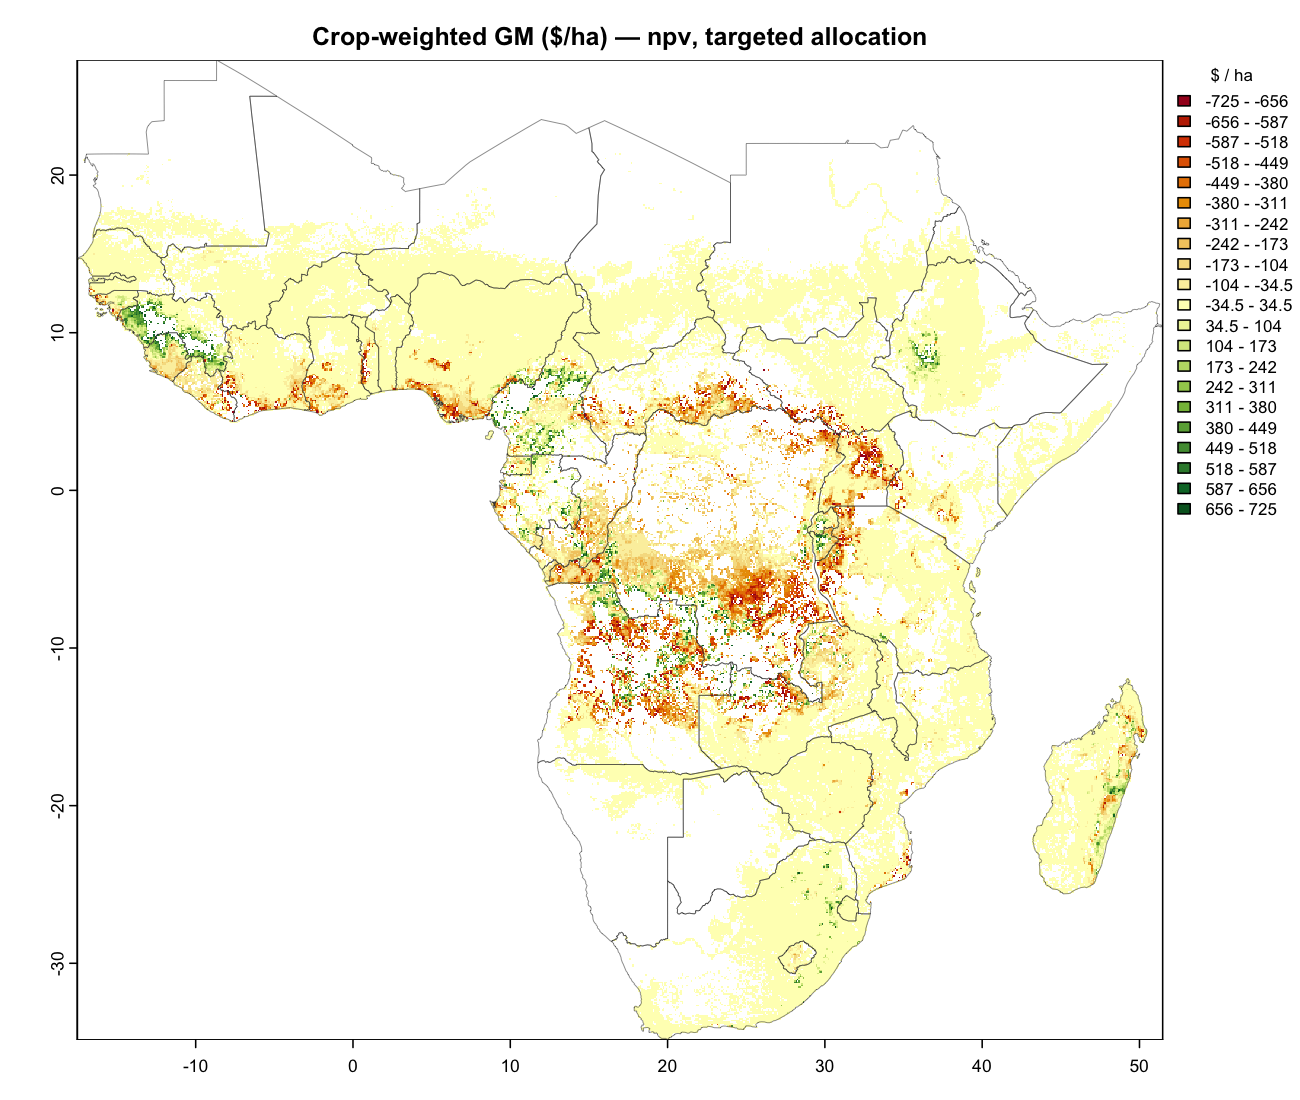
\includegraphics[width=2.6in,height=\textheight,keepaspectratio]{maps/profitability/ssa_gm_npv_targeted.png}
&
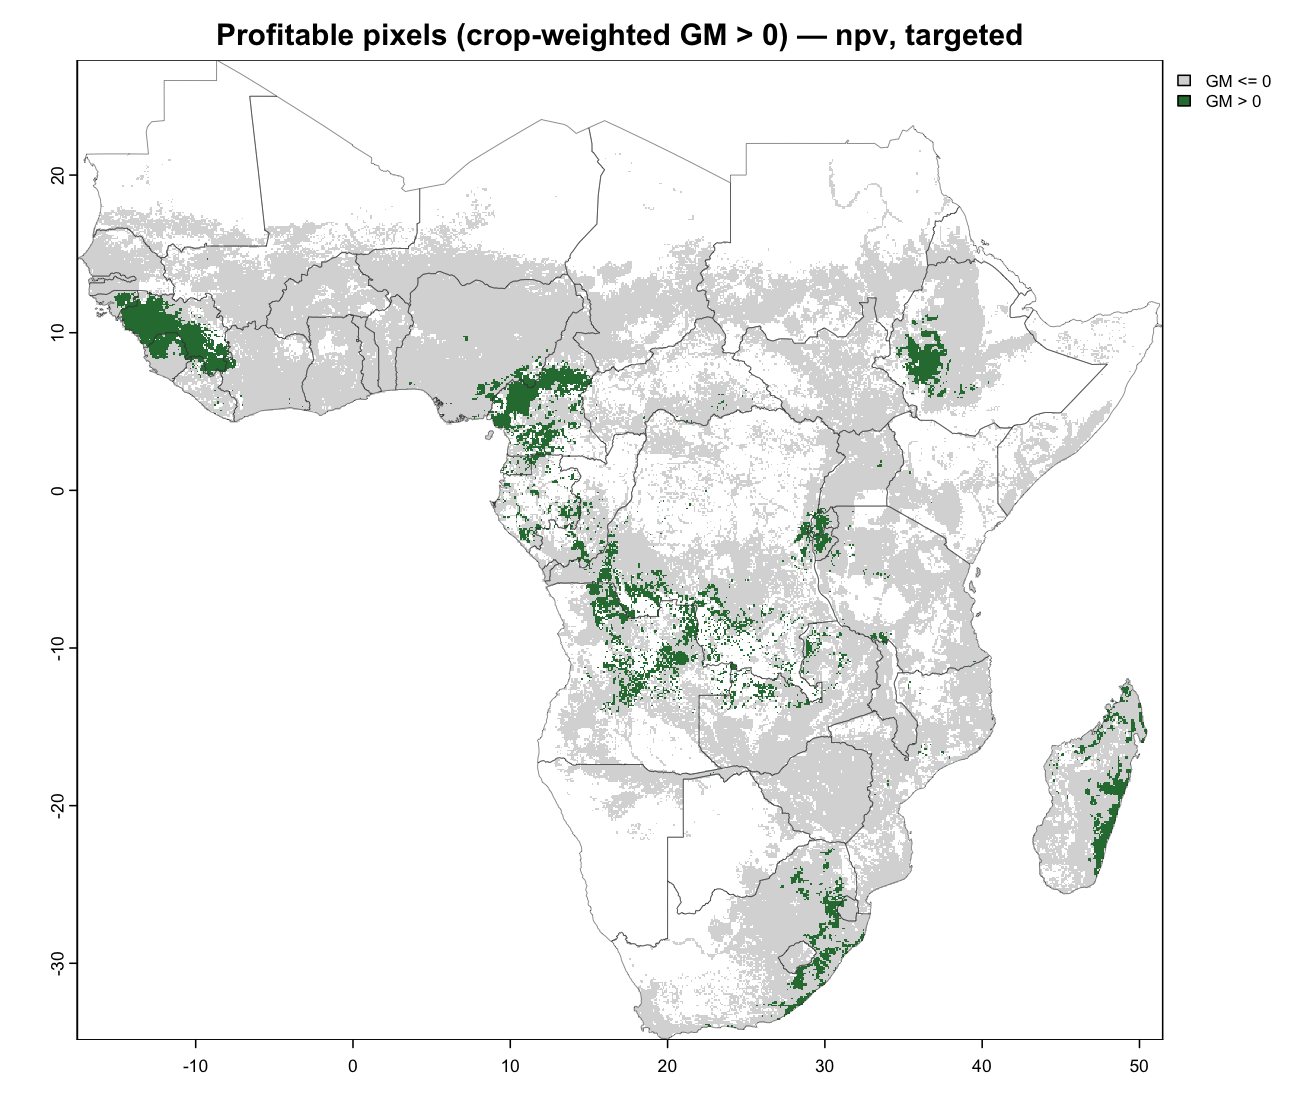
\includegraphics[width=2.6in,height=\textheight,keepaspectratio]{maps/profitability/profitable_mask_npv_targeted.png} \\
\textbf{Breakeven carbon price (NPV, targeted)} & \textbf{Crop-weighted
GM (NPV, uniform 20 t/ha)} \\
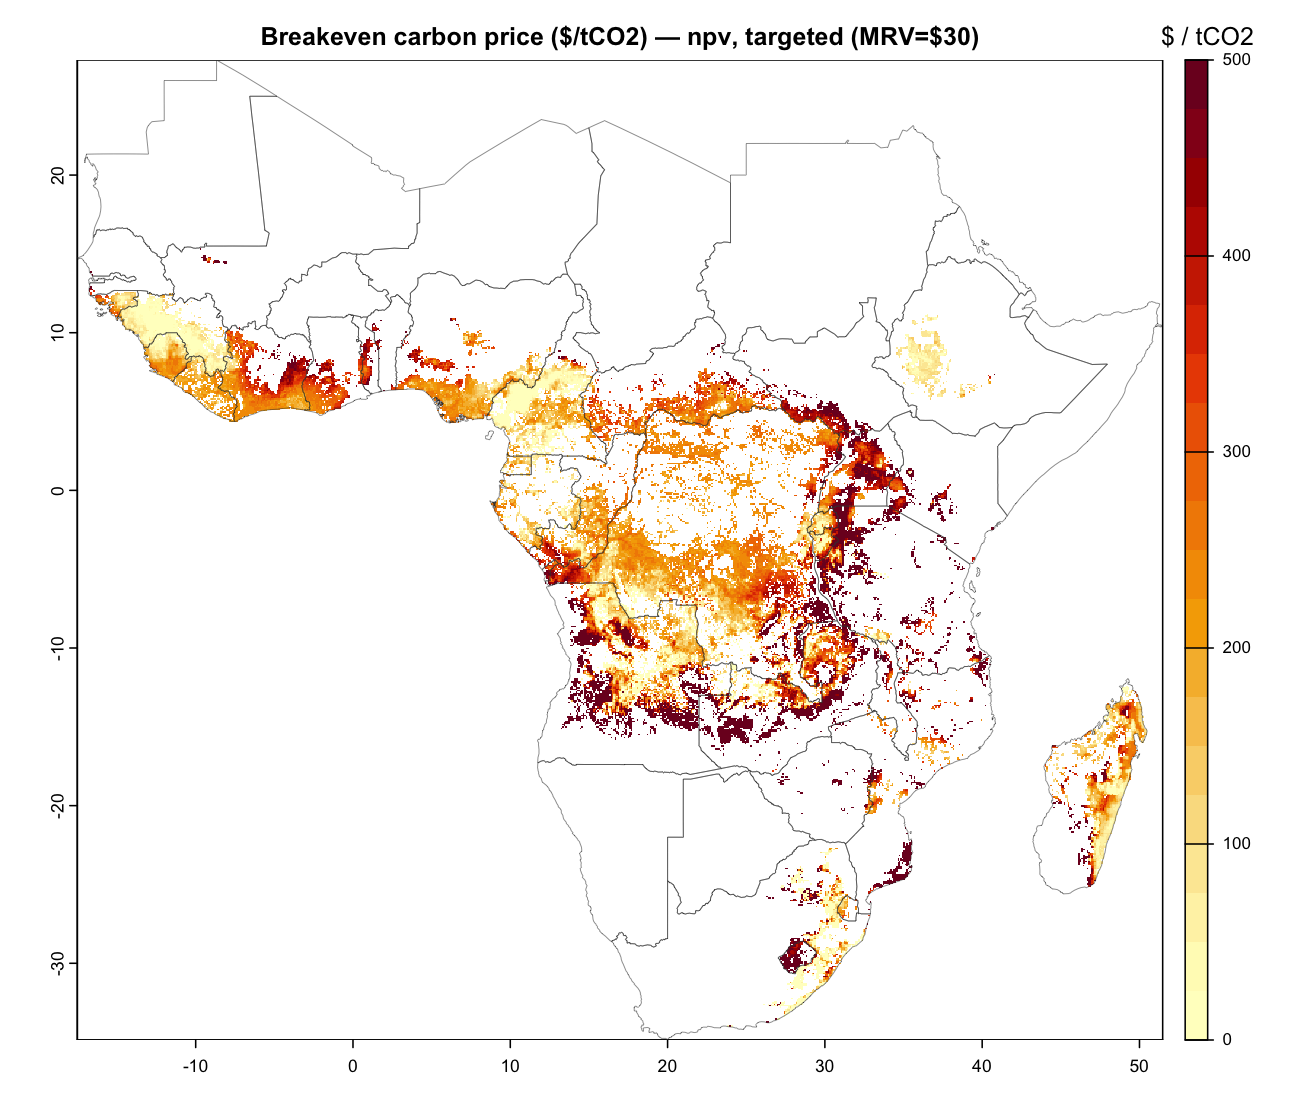
\includegraphics[width=2.6in,height=\textheight,keepaspectratio]{maps/profitability/breakeven_carbon_npv_targeted.png}
&
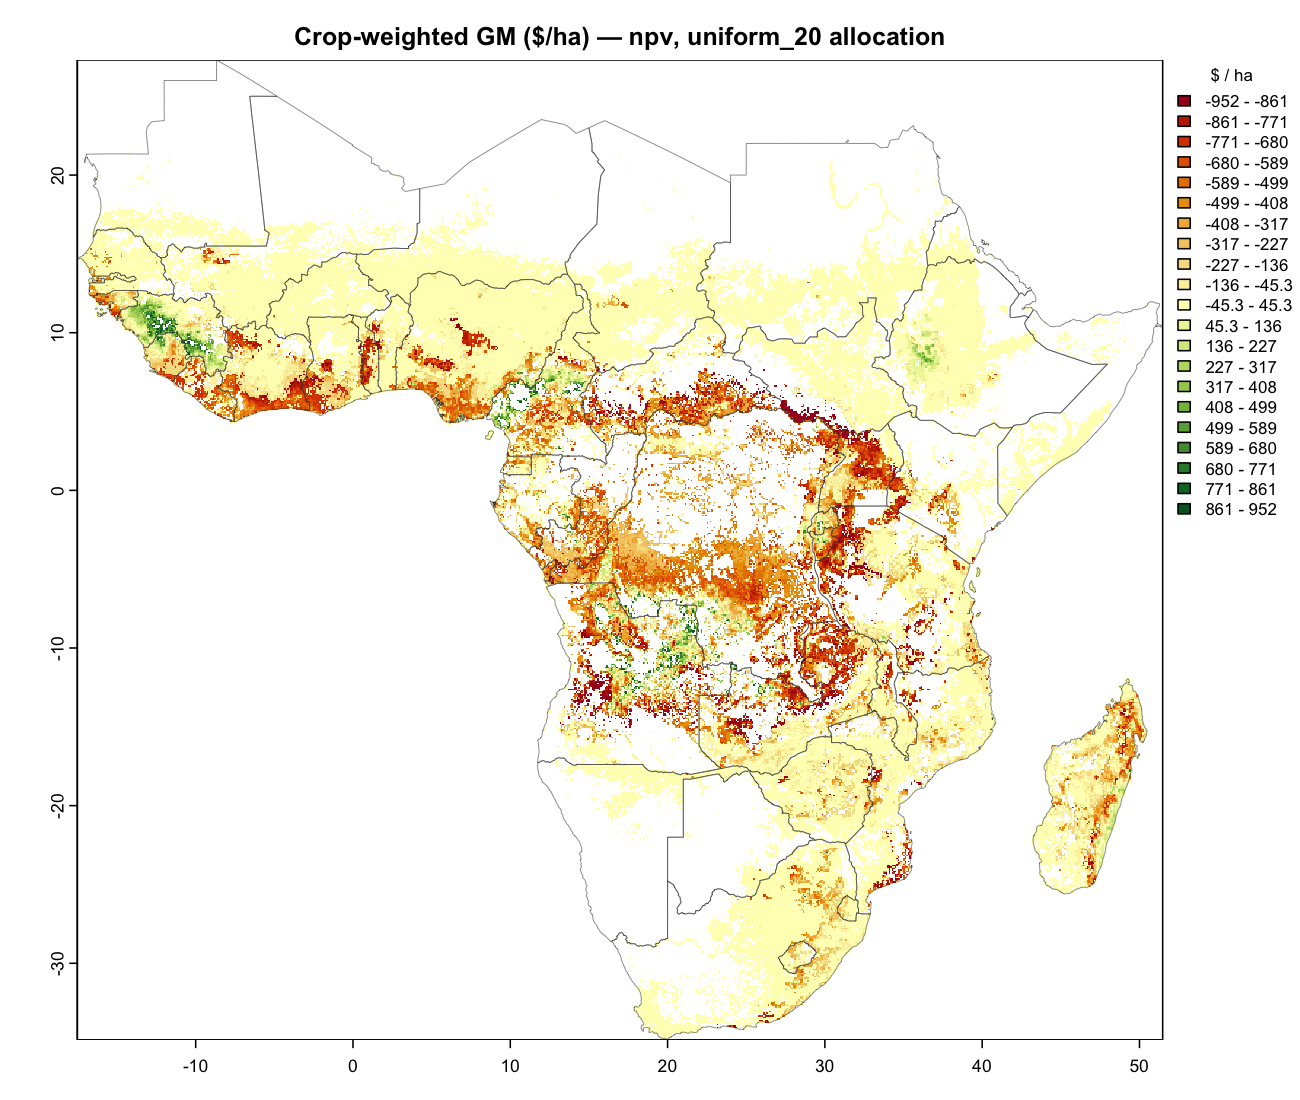
\includegraphics[width=2.6in,height=\textheight,keepaspectratio]{maps/profitability/ssa_gm_npv_uniform_20.png} \\
\end{longtable}
}

\subsubsection{7.2 SSA-wide totals under different assumptions
(refreshed
2026-05-26)}\label{ssa-wide-totals-under-different-assumptions-refreshed-2026-05-26}

Source: \texttt{docs/tables/output-ssa-summary.csv} --- one row per
regime × allocation. Refreshed 2026-05-26 after the round-1 conservatism
review landed (grain 50 µm, MRV \$20/tCO₂, year-1 agronomic summed over
5-yr horizon, CGIAR-CSI Global Aridity Index, per-crop EcoCrop max-pH).

\begin{small}

{\def\LTcaptype{none} % do not increment counter
\begin{longtable}[]{@{}
  >{\raggedright\arraybackslash}p{(\linewidth - 16\tabcolsep) * \real{0.1111}}
  >{\raggedright\arraybackslash}p{(\linewidth - 16\tabcolsep) * \real{0.1111}}
  >{\raggedleft\arraybackslash}p{(\linewidth - 16\tabcolsep) * \real{0.1111}}
  >{\raggedleft\arraybackslash}p{(\linewidth - 16\tabcolsep) * \real{0.1111}}
  >{\raggedleft\arraybackslash}p{(\linewidth - 16\tabcolsep) * \real{0.1111}}
  >{\raggedleft\arraybackslash}p{(\linewidth - 16\tabcolsep) * \real{0.1111}}
  >{\raggedleft\arraybackslash}p{(\linewidth - 16\tabcolsep) * \real{0.1111}}
  >{\raggedleft\arraybackslash}p{(\linewidth - 16\tabcolsep) * \real{0.1111}}
  >{\raggedleft\arraybackslash}p{(\linewidth - 16\tabcolsep) * \real{0.1111}}@{}}
\toprule\noalign{}
\begin{minipage}[b]{\linewidth}\raggedright
Regime
\end{minipage} & \begin{minipage}[b]{\linewidth}\raggedright
Allocation
\end{minipage} & \begin{minipage}[b]{\linewidth}\raggedleft
Total GM (M\$)
\end{minipage} & \begin{minipage}[b]{\linewidth}\raggedleft
Agro (M\$)
\end{minipage} & \begin{minipage}[b]{\linewidth}\raggedleft
Basalt (M\$)
\end{minipage} & \begin{minipage}[b]{\linewidth}\raggedleft
CDR rev. (M\$)
\end{minipage} & \begin{minipage}[b]{\linewidth}\raggedleft
CDR (Mt)
\end{minipage} & \begin{minipage}[b]{\linewidth}\raggedleft
Profitable (Mha)
\end{minipage} & \begin{minipage}[b]{\linewidth}\raggedleft
CDR on profitable (Mt)
\end{minipage} \\
\midrule\noalign{}
\endhead
\bottomrule\noalign{}
\endlastfoot
\textbf{year-1} & \textbf{targeted} & \textbf{+18,440} & 30,220 & 21,545
& 10,566 & 81.3 & 137.9 & 58.4 \\
NPV & targeted & −1,107 & 12,030 & 21,545 & 8,391 & 81.3 & 132.4 &
37.4 \\
\textbf{equilibrium} & \textbf{targeted} & \textbf{+1,965} & 6,044 &
7,364 & 3,442 & 26.5 & 134.9 & 13.6 \\
\textbf{year-1} & \textbf{uniform 10} & \textbf{+19,950} & 30,220 &
75,918 & 13,742 & 105.7 & 127.1 & 81.6 \\
NPV & uniform 10 & −6,106 & 5,495 & 75,918 & 10,914 & 105.7 & 119.2 &
68.3 \\
equilibrium & uniform 10 & −4,200 & 6,044 & 75,918 & 13,742 & 105.7 &
120.6 & 71.0 \\
\textbf{year-1} & \textbf{uniform 20} & \textbf{+9,712} & 30,220 &
151,836 & 27,485 & 211.4 & 124.1 & 153.7 \\
NPV & uniform 20 & −17,701 & 5,495 & 151,836 & 21,827 & 211.4 & 117.4 &
130.4 \\
equilibrium & uniform 20 & −14,439 & 6,044 & 151,836 & 27,485 & 211.4 &
118.6 & 135.4 \\
year-1 & uniform 50 & −21,002 & 30,220 & 379,591 & 68,712 & 528.6 &
120.6 & 355.1 \\
NPV & uniform 50 & −52,486 & 5,495 & 379,591 & 54,567 & 528.6 & 116.1 &
314.6 \\
equilibrium & uniform 50 & −45,153 & 6,044 & 379,591 & 68,712 & 528.6 &
117.1 & 325.4 \\
\end{longtable}
}

\end{small}

Read across: the \textbf{year-1 targeted} row now leads at
\textbf{\$18.4 B} total SSA-wide GM (up from −\$13.9 B pre-refresh) on
137.9 Mha profitable area --- the horizon-summed agronomic side now
scales with 5× annual agronomic returns. \textbf{Year-1 uniform 10} is
the highest absolute total (\$20.0 B) because basalt is applied across
all cropland regardless of acidity, and the new max-pH cliffs make most
of that cropland agronomically responsive. The \textbf{NPV-targeted} row
is now only mildly negative (−\$1.1 B vs.~−\$9.8 B before) --- most of
the headline gap closed once the unit mismatch in year-1 was fixed; the
residual −\$1 B reflects the 10 \% discount rate eating into both
revenue streams. \textbf{Equilibrium-targeted} is solidly positive (+\$2
B) at a 26.5 Mt CDR footprint. Uniform-50 stays negative across all
regimes --- 50 t/ha on every cropland pixel is excess basalt where it
isn't needed, and the deep-tail cost dominates. The full per-country and
per-crop breakdowns are in \texttt{docs/erw-results.pdf}. The same CSVs
feed \texttt{erw-supply.R}'s ranking.

\begin{center}\rule{0.5\linewidth}{0.5pt}\end{center}

\subsection{8. Parameters and constants}\label{parameters-and-constants}

See \texttt{docs/erw-parameters.md} for the full catalogue with
citations, source URLs and DOIs. The blocks in §6 above repeat only the
constants that materially set the headline result; the parameters doc is
authoritative for everything else.

Quick reference of the six \textbf{decision variables} (the only knobs
swept by \texttt{erw-8}):

{\def\LTcaptype{none} % do not increment counter
\begin{longtable}[]{@{}
  >{\raggedright\arraybackslash}p{(\linewidth - 6\tabcolsep) * \real{0.2500}}
  >{\raggedright\arraybackslash}p{(\linewidth - 6\tabcolsep) * \real{0.2500}}
  >{\raggedright\arraybackslash}p{(\linewidth - 6\tabcolsep) * \real{0.2500}}
  >{\raggedright\arraybackslash}p{(\linewidth - 6\tabcolsep) * \real{0.2500}}@{}}
\toprule\noalign{}
\begin{minipage}[b]{\linewidth}\raggedright
Decision variable
\end{minipage} & \begin{minipage}[b]{\linewidth}\raggedright
Default
\end{minipage} & \begin{minipage}[b]{\linewidth}\raggedright
Where set
\end{minipage} & \begin{minipage}[b]{\linewidth}\raggedright
Sweep range
\end{minipage} \\
\midrule\noalign{}
\endhead
\bottomrule\noalign{}
\endlastfoot
\texttt{CaO\_frac}, \texttt{MgO\_frac} (feedstock) & 0.10 / 0.07 &
\texttt{erw-3} & not currently swept \\
\texttt{grain\_size\_um} & \textbf{50 µm} & \texttt{erw-3} & 10 / 30 /
50 / 100 / 200 / 500 µm \\
\texttt{allocation} & LiTAS-targeted & \texttt{erw-7}, \texttt{erw-8} &
+ uniform 10 / 20 / 50 \\
\texttt{CARBON\_PRICE\_USD\_T} & \$150 / tCO₂ & \texttt{erw-7},
\texttt{erw-8} & swept jointly with crop + basalt price \\
\texttt{MRV\_COST\_USD\_T\_CO2} & \textbf{\$20 / tCO₂} & \texttt{erw-7},
\texttt{erw-8} & 0 -- 80 \$ / tCO₂ \\
\texttt{DISCOUNT\_RATE\_PCT} & 10 \% & \texttt{erw-7} & NPV regime
only \\
\end{longtable}
}

\begin{center}\rule{0.5\linewidth}{0.5pt}\end{center}

\subsection{9. Validation and known
issues}\label{validation-and-known-issues}

\subsubsection{What has been
sanity-checked}\label{what-has-been-sanity-checked}

\begin{itemize}
\tightlist
\item
  B1 pH map matches the qualitative expectation for SSA (acidic in humid
  tropics, alkaline in Sahel and parts of southern Africa).
\item
  B3 CDR-yield map is strongest in the humid tropics (Guinea, Congo
  basin) and suppressed in the Sahel --- the expected pattern given
  climate scaling and the aridity-driven pedogenic-C deduction.
\item
  B4 delivered-price map shows the expected geography --- cheap near
  basalt outcrops (Ethiopian highlands, East African Rift, Cameroon
  volcanic line, Madagascar, southern Africa), capped at \$50 / t across
  West Africa and the Sahel.
\item
  B4 source-mask polygon counts match the GLiM v1 catalogue (5,266 vb +
  1,189 pb in SSA).
\end{itemize}

\subsubsection{Open issues}\label{open-issues}

{\def\LTcaptype{none} % do not increment counter
\begin{longtable}[]{@{}
  >{\raggedright\arraybackslash}p{(\linewidth - 6\tabcolsep) * \real{0.2500}}
  >{\raggedright\arraybackslash}p{(\linewidth - 6\tabcolsep) * \real{0.2500}}
  >{\raggedright\arraybackslash}p{(\linewidth - 6\tabcolsep) * \real{0.2500}}
  >{\raggedright\arraybackslash}p{(\linewidth - 6\tabcolsep) * \real{0.2500}}@{}}
\toprule\noalign{}
\begin{minipage}[b]{\linewidth}\raggedright
Issue
\end{minipage} & \begin{minipage}[b]{\linewidth}\raggedright
Severity
\end{minipage} & \begin{minipage}[b]{\linewidth}\raggedright
Block
\end{minipage} & \begin{minipage}[b]{\linewidth}\raggedright
Mitigation
\end{minipage} \\
\midrule\noalign{}
\endhead
\bottomrule\noalign{}
\endlastfoot
Bayesian yield arm not fit & high (limits scenario realism) & B6 & run
\texttt{erw-yield-fit.R} once \texttt{brms} + Stan are installed; the
trial dataset is the bottleneck, not the code \\
\texttt{erw-7} profitability not run & high (no headline output yet) &
B7 & all inputs are in place; one run suffices \\
\texttt{erw-supply}, \texttt{erw-8} not run & medium & B8, B9 & both
depend on B7 \\
Industrial by-products not modelled & medium (regional realism) & B4 &
requires a separate inventory of steel mills, cement plants, mine
tailings \\
Ultramafic outcrops excluded from feedstock & low (intentional) & B4 &
mark them explicitly in a future ``rejected feedstock'' overlay \\
MRV cost is constant \$30 / tCO₂ regardless of scale or protocol & low &
B7 & sweep already covers 0 -- 80 \$; consider scale-dependence in a
future revision \\
Pedogenic-C deduction uses MAP only, not full AI & low & B3 & switch to
AI = MAP / PET when a PET surface is available \\
14-row trial dataset is prior-dominated & medium & B6 (Bayesian arm) &
append trials as new evidence appears (Beerling group, InPlanet, Flux
trials) \\
Single-currency model & low & all & USD throughout; not a problem for
ex-ante analysis \\
\end{longtable}
}

\begin{center}\rule{0.5\linewidth}{0.5pt}\end{center}

\subsection{10. How to reproduce}\label{how-to-reproduce}

\subsubsection{10.1 Environment}\label{environment}

\begin{Shaded}
\begin{Highlighting}[]
\CommentTok{\# R 4.5+, with the geodata, terra, sf, here, brms, malariaAtlas packages}
\ExtensionTok{Rscript}\NormalTok{ erw/erw{-}0{-}install{-}packages.R}
\end{Highlighting}
\end{Shaded}

LaTeX is needed only for the framework + pipeline figures
(\texttt{pdflatex} + \texttt{pdftocairo}).

\subsubsection{10.2 Run order}\label{run-order}

\begin{Shaded}
\begin{Highlighting}[]
\CommentTok{\# 1. inputs and working grid}
\ExtensionTok{Rscript}\NormalTok{ erw/erw{-}1{-}layers{-}soilgrids.R}
\ExtensionTok{Rscript}\NormalTok{ erw/erw{-}2{-}layers{-}spam.R}

\CommentTok{\# 2. basalt requirements}
\ExtensionTok{Rscript}\NormalTok{ erw/erw{-}3{-}basalt{-}requirements.R}

\CommentTok{\# 3. crop response}
\ExtensionTok{Rscript}\NormalTok{ erw/erw{-}4{-}crop{-}parameters.R}
\ExtensionTok{Rscript}\NormalTok{ erw/erw{-}5{-}crop{-}yield{-}loss{-}function.R}

\CommentTok{\# 4. CDR + cost surfaces}
\ExtensionTok{Rscript}\NormalTok{ erw/erw{-}9{-}cdr{-}yield.R}
\ExtensionTok{Rscript}\NormalTok{ erw/erw{-}energy{-}country.R}
\ExtensionTok{Rscript}\NormalTok{ erw/erw{-}fetch{-}friction{-}surface.R   }\CommentTok{\# one{-}off — pulls MAP friction}
\ExtensionTok{Rscript}\NormalTok{ erw/erw{-}basalt{-}access.R}

\CommentTok{\# 5. (optional) Bayesian yield arm}
\ExtensionTok{Rscript}\NormalTok{ erw/erw{-}yield{-}fit.R}
\ExtensionTok{Rscript}\NormalTok{ erw/erw{-}yield{-}predict.R}

\CommentTok{\# 6. profitability, supply, sensitivity}
\ExtensionTok{Rscript}\NormalTok{ erw/erw{-}7{-}profitability{-}function.R}
\ExtensionTok{Rscript}\NormalTok{ erw/erw{-}supply.R}
\ExtensionTok{Rscript}\NormalTok{ erw/erw{-}8{-}sensitivity{-}analysis.R}

\CommentTok{\# 7. render maps, results, and rebuild figures}
\ExtensionTok{Rscript}\NormalTok{ erw/erw{-}plot{-}maps.R                      }\CommentTok{\# 12 indicator maps}
\ExtensionTok{Rscript}\NormalTok{ erw/erw{-}10{-}profitability{-}maps{-}tables.R   }\CommentTok{\# profitability maps + 3 CSV tables}
\ExtensionTok{pdflatex}\NormalTok{ docs/erw{-}pipeline{-}flow.tex }\DataTypeTok{\textbackslash{}}
  \KeywordTok{\&\&} \ExtensionTok{pdftocairo} \AttributeTok{{-}svg}\NormalTok{ docs/erw{-}pipeline{-}flow.pdf docs/erw{-}pipeline{-}flow.svg}
\ExtensionTok{pdflatex}\NormalTok{ docs/erw{-}conceptual{-}framework.tex }\DataTypeTok{\textbackslash{}}
  \KeywordTok{\&\&} \ExtensionTok{pdftocairo} \AttributeTok{{-}svg}\NormalTok{ docs/erw{-}conceptual{-}framework.pdf docs/erw{-}conceptual{-}framework.svg}

\CommentTok{\# 8. rebuild documentation PDFs}
\FunctionTok{bash}\NormalTok{ docs/build{-}erw{-}model.sh}
\FunctionTok{bash}\NormalTok{ docs/build{-}erw{-}results.sh}
\FunctionTok{bash}\NormalTok{ docs/build{-}erw{-}tutorial.sh}
\end{Highlighting}
\end{Shaded}

\subsubsection{10.3 Expected runtimes (Apple Silicon, single
core)}\label{expected-runtimes-apple-silicon-single-core}

{\def\LTcaptype{none} % do not increment counter
\begin{longtable}[]{@{}
  >{\raggedright\arraybackslash}p{(\linewidth - 2\tabcolsep) * \real{0.5000}}
  >{\raggedright\arraybackslash}p{(\linewidth - 2\tabcolsep) * \real{0.5000}}@{}}
\toprule\noalign{}
\begin{minipage}[b]{\linewidth}\raggedright
Stage
\end{minipage} & \begin{minipage}[b]{\linewidth}\raggedright
Time
\end{minipage} \\
\midrule\noalign{}
\endhead
\bottomrule\noalign{}
\endlastfoot
\texttt{erw-1}, \texttt{erw-2} (downloads + resampling) &
\textasciitilde30 -- 60 min first time, cached afterwards \\
\texttt{erw-3}, \texttt{erw-9} & a few minutes each \\
\texttt{erw-fetch-friction-surface} & 5 -- 10 min (one-off download) \\
\texttt{erw-basalt-access} (costDist) & \textasciitilde10 min \\
\texttt{erw-7}, \texttt{erw-8} & minutes -- hours depending on sweep
depth \\
\texttt{erw-plot-maps} (12 maps) & \textasciitilde15 min \\
\texttt{erw-10-profitability-maps-tables} (48 maps + 3 CSVs) &
\textasciitilde5 min \\
\end{longtable}
}

\begin{center}\rule{0.5\linewidth}{0.5pt}\end{center}

\subsection{11. Gaps and roadmap}\label{gaps-and-roadmap}

\subsubsection{Near-term (within current
month)}\label{near-term-within-current-month}

\begin{enumerate}
\def\labelenumi{\arabic{enumi}.}
\tightlist
\item
  Fit the Bayesian yield arm (\texttt{erw-yield-fit.R}) once
  \texttt{brms} + Stan are installed locally.
\item
  Run \texttt{erw-7} end-to-end to produce the 276-raster profitability
  stack \texttt{\{crop\}\_\{regime\}.tif} under
  \texttt{economics\_erw/\{allocation\}/}.
\item
  Run \texttt{erw-supply} and \texttt{erw-8} and render their headline
  figures.
\item
  Add indicator maps for the supply curves and the year-1 / NPV /
  equilibrium profitability comparison.
\end{enumerate}

\subsubsection{Medium-term}\label{medium-term}

\begin{enumerate}
\def\labelenumi{\arabic{enumi}.}
\setcounter{enumi}{4}
\tightlist
\item
  \textbf{Industrial by-product feedstock layer.} Inventory of steel
  mills (GEM Steel Plant Tracker), cement-clinker plants (Global Cement
  Directory), and active mine tailings (USGS / national geological
  surveys). Add a point-source feedstock layer and feedstock- chemistry
  table; rerun B4 with the union of mafic outcrops and by-product
  points.
\item
  \textbf{Cross-country MRV cost differentiation.} Some jurisdictions
  (Brazil, Kenya) have simpler smallholder-aggregator pathways; the flat
  \$30 / tCO₂ assumption over-estimates cost for those.
\item
  \textbf{Aridity index using AI = MAP / PET} instead of MAP-only for
  the pedogenic-C deduction. Requires a PET surface (CGIAR-CSI or
  computed from WorldClim).
\end{enumerate}

\subsubsection{Long-term}\label{long-term}

\begin{enumerate}
\def\labelenumi{\arabic{enumi}.}
\setcounter{enumi}{7}
\tightlist
\item
  \textbf{Multi-feedstock decision rule.} Currently feedstock chemistry
  is fixed; the user chooses one. Generalise to a per-pixel
  cheapest-eligible-feedstock rule given a chemistry inventory.
\item
  \textbf{Time-resolved deployment scenarios.} Year-by-year deployment
  under supply caps, carbon-price paths, and yield-learning curves.
\item
  \textbf{Smallholder-aggregator economic model.} Costs and revenues at
  the aggregator level (transport, MRV pooling, finance) rather than the
  per-pixel ``farmer'' level.
\end{enumerate}

\begin{center}\rule{0.5\linewidth}{0.5pt}\end{center}

\subsection{12. References}\label{references}

The full bibliography is in \texttt{docs/erw-review.md}. The most
load-bearing citations are:

\begin{itemize}
\tightlist
\item
  Beerling, D. J. et al.~(2020). \emph{Potential for large-scale CO₂
  removal via enhanced rock weathering with croplands.} \textbf{Nature}
  583, 242 -- 248.
\item
  Strefler, J. et al.~(2018). \emph{Potential and costs of carbon
  dioxide removal by enhanced weathering of rocks.} \textbf{ERL} 13,
  034010.
\item
  Lewis, A. L. et al.~(2021). \emph{Effects of mineralogy, chemistry and
  physical properties of basalts on carbon capture potential and
  plant-nutrient element release via enhanced weathering.}
  \textbf{Applied Geochemistry} 132, 105023.
  doi:10.1016/j.apgeochem.2021.105023. (Reference for the
  reactive-fraction calibration used in \texttt{erw-3}.)
\item
  Hartmann, J. \& Moosdorf, N. (2012). \emph{The new global lithological
  map database GLiM.} PANGAEA doi:10.1594/PANGAEA.788537.
\item
  Weiss, D. J. et al.~(2018). \emph{A global map of travel time to
  cities to assess inequalities in accessibility in 2015.}
  \textbf{Nature} 553, 333--336. doi:10.1038/nature25181.
\item
  Weiss, D. J. et al.~(2020). \emph{Global maps of travel time to
  healthcare facilities.} \textbf{Nature Medicine} 26, 1835--1838.
  doi:10.1038/s41591-020-1059-1. (Source of the Malaria Atlas Project
  2019 motorised friction surface used in \texttt{erw-basalt-access}.)
\item
  Aramburu Merlos, F., Silva, J. V., Baudron, F. \& Hijmans, R. J.
  (2023). \emph{Estimating lime requirements for tropical soils: Model
  comparison and development.} \textbf{Geoderma} 432,

  \begin{enumerate}
  \def\labelenumi{\arabic{enumi}.}
  \setcounter{enumi}{116420}
  \tightlist
  \item
    (Reference for the LiTAS lime-equivalence recipe used in
    \texttt{erw-3}.)
  \end{enumerate}
\item
  Kanzaki, Y., Planavsky, N. J. \& Reinhard, C. T. (2023). \emph{New
  estimates of the storage permanence and ocean co-benefits of enhanced
  rock weathering.} \textbf{PNAS Nexus} 2 (4), pgad059.
\item
  Beerling, D. J. et al.~(2024). \emph{Enhanced weathering in the US
  Corn Belt delivers carbon removal with agronomic benefits.}
  \textbf{PNAS} 121 (9), e2319436121.
\item
  Haque, F. et al.~(2025). \emph{Agronomic Performance of Enhanced Rock
  Weathering in a Tropical Smallholder System: A Maize Trial in Kenya.}
  CDRXIV preprint 410 (Flux Carbon / UNCCD).
\item
  Dupla, X., Bertagni, M. B. \& Grand, S. (2025). \emph{Three Years of
  Field Trials Indicate a Sustained Enhanced Rock Weathering Signal with
  Limited CO₂ Removal.} \textbf{Environmental Science \& Technology} 59
  (48), 25751--25764.
\end{itemize}

\begin{center}\rule{0.5\linewidth}{0.5pt}\end{center}

\emph{This document is the canonical state of the model. When you change
a script, a constant, a data source, or an output, edit the relevant
block under §6 and add a dated entry to §1. Anything that is not in this
document --- even if it lives in the code --- is not part of the model's
documented behaviour.}

\end{document}
